\section*{Introduction}

Understanding markets is one of the major issues in game theory. It has implications in human economical markets \citep{osborne_bargaining_1990,chade_sorting_2017}, as well as in biological markets \citep{noe_biological_1995,hammerstein_biological_2016,fruteau_supply_2009,baumard_mutualistic_2013}. Search and matching models have a very important place in the market literature. The general principle is as follows: individuals meet two by two and may decide to interact for a certain period of time and generate benefits. These models are widely used to try to predict a fundamental property of markets: who interacts with whom. This question is also called the \textit{matching problem}.

Shimer and Smith have written two seminal articles \citep{shimer_assortative_2000,smith_marriage_2006} in this field, in which they (1) assume that individuals vary in their ability to generate benefits and (2) study who interacts with whom when everyone play the equilibrium strategy. More precisely, they derive the conditions for which more productive individuals interact with other productive individuals. This situation is also called a Positive Assortative Matching (PAM).

Both articles address this question, but differ in the way individuals exchange services. In Smith's article \citep{smith_marriage_2006}, each individual receives a payoff that depends on both types. This case is called Non-Transferable Utility (NTU). In Shimer and Smith's article \citep{shimer_assortative_2000}, two individuals generate a benefit whose size depends on the two types and, then, they split the benefit. We decided to replicate results from both articles since the models are so similar.

The authors use game theory to derive the equilibrium, namely the optimal strategy that agents should adopt in a market situation. However, the equilibrium is defined by three rather complex equations for which it is not possible to obtain a closed-form solution. The authors use an algorithm to find numerical solutions which is derived from the proof of the existence of an equilibrium (discussed in \citep{smith_frictional_2011}). We contacted the authors and had access to the code (Mathematica script) used for the first reference article \citep{shimer_assortative_2000}. Although the numerical solutions are mostly illustrative in the two reference articles, similar algorithms have been used in works which aim at fitting these models on actual data \citep{hagedorn_identifying_2017,lise_matching_2016}. This is why we think it is important to replicate the results and have an openly available version of this algorithm for the scientific community. We are able to replicate all figures from both papers, except for one, which is discussed in \textit{Results}.




\section*{Methods}

\subsection*{Model description}

We start by describing the model proposed in the first reference article \citep{shimer_assortative_2000}. In a population of arbitrary size, each individual is defined by a type $x \in [0,1]$. The continuous distribution of types is given by the density function $l$. At any time, an individual is either matched with a partner, or unmatched. An unmatched individual encounters another one at rate $\rho$, and a pair of matched individuals splits at rate $\delta$. The distribution of types for unmatched individuals is given by the \textbf{unmatched density function} $u$.

In the first reference article \citep{shimer_assortative_2000}, the utility in transferable (TU): a pair of individuals generates a benefit of size $f(x,y)$ which is then split with a classic Nash bargaining procedure \citep{osborne_bargaining_1990,shimer_assortative_2000}. The benefit generated $f(x,y)$ is an increasing function of both types $x$ and $y$. Individuals discount time at rate $r$.

Each individual must choose a strategy which consists of saying which types she is willing to accept as a partner. At the equilibrium, all individuals of the same type have the same strategy. We define the \textbf{matching set} function $\alpha$ such that $\alpha(x,y) = 1$ if individuals of type $x$ accept individuals of type $y$ as partners and if types $y$ also accept types $x$. Otherwise, $\alpha(x,y) = 0$. Solving the matching problem --who interacts with whom-- is equivalent to finding the equilibrium value of $\alpha$.

Lastly, it is convenient to introduce a function $v$ which represents, for each type, her \textbf{value}, i.e. her expected lifetime payoff when she is in the unmatched state. The optimal strategy is then clear: an individual should accept a partner if the payoff she will get from this interaction is higher than her unmatched payoff.

Shimer and Smith derive a system of three equations which defines a Nash equilibrium. For more details, see the proof in the article (sections 3 and 4 in \citep{shimer_assortative_2000}).

\begin{align*}[left=\empheqlbrace]
	u(x) &= \frac{\delta l(x)}{\delta + \rho \int_{0}^{1} \alpha(x,y) u(y) dy} &&\forall x \in [0,1]\\
	v(x) &= \theta \int_{0}^{1} (f(x,y)-v(x)-v(y)) \alpha(x,y) u(y) dy &&\forall x \in [0,1]\\
	\alpha(x,y) &=
	\begin{cases}
		1, & \text{if } f(x,y) \geq v(x)+v(y)\\
		0, & \text{otherwise}
	\end{cases}
	&&\forall x,y \in [0,1]^2 
\end{align*}
with $\theta = \frac{\rho}{2(r+\delta)}$ 


Unfortunately, it is not possible to derive a closed-form analytical solution. The trick used by Shimer and Smith \citep{shimer_assortative_2000} to get a numerical approximation is to discretize the type space in $n$ types. The problem can then be written in terms of vectors and matrices. Integrals can be approximated by Riemman sums if $n$ is large enough.

\begin{align*}[left=\empheqlbrace]
	u_i &= \frac{\delta l_i}{\delta + \frac{\rho}{n} \sum\limits_{j=1}^{n} \alpha_{i,j} u_j} &&\forall \; 1 \leq i \leq n\\
	v_i &= \frac{\theta}{n} \sum_{j=1}^{n} (f_{i,j}-v_i-v_j) \alpha_{i,j} u_j &&\forall \; 1 \leq i \leq n\\\
	\alpha_{i,j} &=
	\begin{cases}
		1, & \text{if } f_{i,j} \geq v_i+v_j\\
		0, & \text{otherwise}
	\end{cases}
	&&\forall \; 1 \leq i,j \leq n\
\end{align*}


Because we implement the algorithm with the Numpy library, it is convenient to write the system in matrix notation. We use the following notation for column vectors $\vect{u} = (u_i)_{1 \leq i \leq n}$ and for square matrices $\vect{A} = (\alpha_{i,j})_{1 \leq i \leq n, 1 \leq j \leq n}$.





\begin{align}[left=\empheqlbrace]
	&\vect{u} = \frac{\delta \vect{l}}{\delta \vect{J}_{n,1} + \frac{\rho}{n} \vect{A}\vect{u}}\\
	&\left(\vect{A} \diag(\vect{u}) + \vect{I}_n \circ \left(\frac{n}{\theta} \vect{J}_n + \vect{A} \vect{u}\right)\right) \vect{v} = (\vect{F} \circ \vect{A}) \vect{u}
	\tag{2a}\\
	&\vect{A} = \frac{1}{2} \left( \sgn{\left( \vect{F} - \vect{v} \vect{J}_{1,n} - \vect{J}_{n,1} \vect{v}^\top \right)} + \vect{J}_n \right)
	\tag{3a}
\end{align}
 
Here, the symbol $\circ$ denotes the Hadamard product (element-wise product) and the fraction symbol is used in the sense of Hadamard division (element-wise division).
$\vect{I}_i$ is the identity matrix of size $i$ and $\vect{J}_{i,j}$ is the all-ones matrix of dimensions $i \times j$ ($\vect{J}_{i}$ denotes the square all-ones matrix of dimensions $i \times i$).


In the second reference article \citep{smith_marriage_2006}, utility is non-transferable (NTU): an individual in a pair receives a payoff $f(x,y)$ which depends on her type $x$ and her partner's type $y$. Accordingly, her partner receives a payoff $f(y,x)$. The Nash equilibrium, in this case, is determined by

\begin{align*}[left=\empheqlbrace]
	u(x) &= \frac{\delta l(x)}{\delta + \rho \int_{0}^{1} \alpha(x,y) u(y) dy} &&\forall x \in [0,1]\\
	v(x) &= \frac{\int_{0}^{1} f(x,y) \alpha(x,y) u(y) dy}{\psi + \int_{0}^{1} \alpha(x,y) u(y) dy} &&\forall x \in [0,1]\\
	\alpha(x,y) &=
	\begin{cases}
		1, & \text{if } f(x,y) \geq v(x) \text{ and } f(x,y) \geq v(y)\\
		0, & \text{otherwise}
	\end{cases}
	&&\forall x,y \in [0,1]^2 
\end{align*}
with $\psi = \frac{r+\delta}{\rho}$. We can also write these equations using matrix notation. The first equation is the same as $(1)$ and the other two are:

\begin{align}[left=\empheqlbrace]
	\vect{v} &= \frac{(\vect{F} \circ \vect{A})\vect{u}}{n \psi \vect{J}_{n,1} + \vect{A} \vect{u}}
	\tag{2b}\\
	\vect{A} &= \frac{1}{2} \left(\sgn{\left( \vect{F} - \vect{v} \vect{J}_{1,n} \right)} + \vect{J}_n \right) \circ \frac{1}{2} \left(\sgn{\left( \vect{F} - \vect{J}_{n,1} \vect{v}^\top \right)} + \vect{J}_n \right)
	\tag{3b}
\end{align}





\subsection*{Implementation of the algorithm}

The authors use an algorithm to find the equilibrium numerical values of the unmatched densities $\vect{u}$, the values $\vect{v}$ and, most importantly, the matching set $\vect{A}$. The algorithm is derived from the proof of the existence of an equilibrium (see \citep{smith_frictional_2011} for details). The main idea is to start with an initial guess for the matching set $\vect{A}$, then, since one's probability of being unmatched depends on one's type and on the matching strategy of all players, we can update the unmatched densities $\vect{u}$ accordingly. From this, we can update the values of each type $\vect{v}$ and, finally, derive the new optimal matching strategy of each type $\vect{A}$ according to their values. This tatonnement process can be described by the following algorithm:

\begin{enumerate}[start=0]
	\item Initialize $(\vect{u},\vect{v},\vect{A})$
	\item Update $\vect{u}$ by solving $(1)$
	\item Update $\vect{v}$ by solving $(2a)$
	\item Update $\vect{A}$ by solving $(3a)$
	\item If $\vect{A}$ has been modified by Step 3, return to Step 1, else stop the loop.
\end{enumerate}

The algorithm is the same for the NTU case, one should simply replace equation $(2a)$ with $(2b)$, and equation $(3a)$ with $(3b)$.

Although, there is no formal proof that this algorithm converges to the desired equilibrium, in practice, it does in the majority of cases (L. Smith, personal communication). Moreover, if the algorithm converges, by definition, its solution is the desired Nash equilibrium. However, it can happen that the algorithm gives rise to an infinite loop. This comes from the fact that discretization into $n$ types can lead to the existence of mixed strategies (see \citep{hagedorn_identifying_2017}) which we want to avoid here. Therefore, in Step 4 of the algorithm, we also check if the current value of $\vect{A}$ has already occurred, which would indicate an infinite loop. 


\subsection*{Solving the equations}

Equation $(1)$ is actually a system of nonlinear equations. We use a simple fixed-point iteration to obtain a numerical solution with an accuracy of $10^{-12}$ (section 2.10 in \citep{atkinson_introduction_1989}). In the algorithm used in the first reference article \citep{shimer_assortative_2000} communicated by the authors, the system is also solved with a fixed-point iteration with an additional damping factor and the same accuracy.

Shimer and Smith \citep{shimer_assortative_2000} also use a fixed-point iteration for solving $(2a)$. In our implementation, we can take advantage of the fact that $(2a)$ is a system of linear equations and can be written as $\vect{P} \vect{v} = \vect{q}$, with $\vect{P} = \vect{A} \diag(\vect{u}) + \vect{I}_n \circ \left(\frac{n}{\theta} \vect{J}_n + \vect{A} \vect{u}\right)$ and $\vect{q} = (\vect{F} \circ \vect{A}) \vect{u}$. The vector of values $\vect{v}$ is $ \vect{v} = \vect{P}^{-1} \vect{q} $

Finally, equations $(2b)$, $(3a)$ and $(3b)$ are straightforward to solve.

The algorithm is implemented in Python.





\section*{Results}

We were able to replicate almost all results from both reference articles \citep{shimer_assortative_2000,smith_marriage_2006}. Figures \ref{fig:fig1} and \ref{fig:fig2} replicate results from \citep{shimer_assortative_2000} (transferable utility) and Figure \ref{fig:fig3} replicate results from \citep{smith_marriage_2006} (non-transferable utility).

\subsection*{Shimer \& Smith 2000}

Figure \ref{fig:fig1} replicates figure 1 from the first reference article \citep{shimer_assortative_2000}. It shows the matching set $\vect{A}$ at the equilibrium for several values of the number $n$ of discrete types. As $n$ increases, the discrete case converges to the continuous case. All further results (with one exception) are obtained with $n=500$. Note that, in this case, the matching set is such that there is a Positive Assortative Matching (PAM, see \textit{Introduction}): the higher one's type, the higher the minimum type that one is willing to accept as a partner.

Figure \ref{fig:fig2}A, \ref{fig:fig2}B and \ref{fig:fig2}C respectively replicate figures 3a, 3b and figure 4 from \citep{shimer_assortative_2000}. Here, there is no Positive Assortative Matching at the equilibrium. Figure \ref{fig:fig2}B was obtained with $n=501$ because an infinite loop occurs for $n=500$. Note that, with the same parameters, the algorithm also fails to converge when we run the Mathematica script that the authors have provided. Lastly, Figure \ref{fig:fig2}D replicates an extra figure not present in the first reference article \citep{shimer_assortative_2000}, but in \citep{smith_frictional_2011} (figure 4). We have decided to include it to increase the confidence in the robustness of our implementation.



\subsection*{Smith 2006}

Figure \ref{fig:fig3}A and \ref{fig:fig3}B are two attempts at replicating figure 1 from the second reference article \citep{smith_marriage_2006}. When we run our algorithm with the parameters provided in the figure caption in \citep{smith_marriage_2006}, replication fails (Fig.~\ref{fig:fig3}A). Indeed, by comparing Figure \ref{fig:fig3}A and figure 1 from \citep{smith_marriage_2006}, one can see that the resulting matching sets are qualitatively different. We do not have access to the code which has been used in this article because it was lost (L. Smith, personal communication). Thus, it is not possible to know where the discrepancy between the results comes from. Nevertheless, we would like propose an explanation for this discrepancy. Please note that \textbf{this is entirely speculative, since there is no way to run the exact algorithm} used in \citep{smith_marriage_2006}. The caption of figure 1 in \citep{smith_marriage_2006} specifies that the author used ``$\delta=.1$'', which usually means ``$0.1$''. Still, this notation is not used for the parameter ``$r=0.3$''. We think that there might be a typo in ``$\delta=.1$''\footnote{Note that a slightly different version of the second reference article \citep{smith_marriage_2006} was previously published in the \textit{Social Science Research Network} in 1997 \citep{smith_marriage_1997}. However, the parameter values given in the figure caption are identical.}. We run the algorithm for $\delta=1.1$ and the resulting figure (Fig.~\ref{fig:fig3}B) seems to replicate figure 1 from \citep{smith_marriage_2006}.

In Figure \ref{fig:fig3}C, were able to replicate figure 2 of \citep{smith_marriage_2006}. However, in \citep{smith_marriage_2006}, the caption below figure 2 states that ``the parameters in fig.~1 are assumed, except $\rho=3$''. We therefore use $\delta=0.1$;, which leads to a good replicate of figure 2 from \citep{smith_marriage_2006}. Changing $\delta$ to $1.1$, as we did for the previous figure, would lead to a replication failure (results not shown).


\subsection*{Gaussian distribution}

In both reference articles, the distribution of types is always assumed to be uniform, i.e. $\forall x \in [0,1] \ : \ l(x)=1$. This is not necessarily the case in real-life applications of search and matching models (see \citep{hagedorn_identifying_2017}). In Figure \ref{fig:fig4}, we show an example of matching sets at the equilibrium for the transferable utility case with a Gaussian distribution of types. There is no replication purpose for this result, but we think it might be useful to include it given the importance of this assumption.

\def \smallScl {0.15}
\def \mediumScl {0.2}
\def \largeScl {0.3}



\begin{figure}[!ht]
	\centering
	\subfloat{\stackinset{c}{}{t}{-.2in}{$\bm{n=10}$}{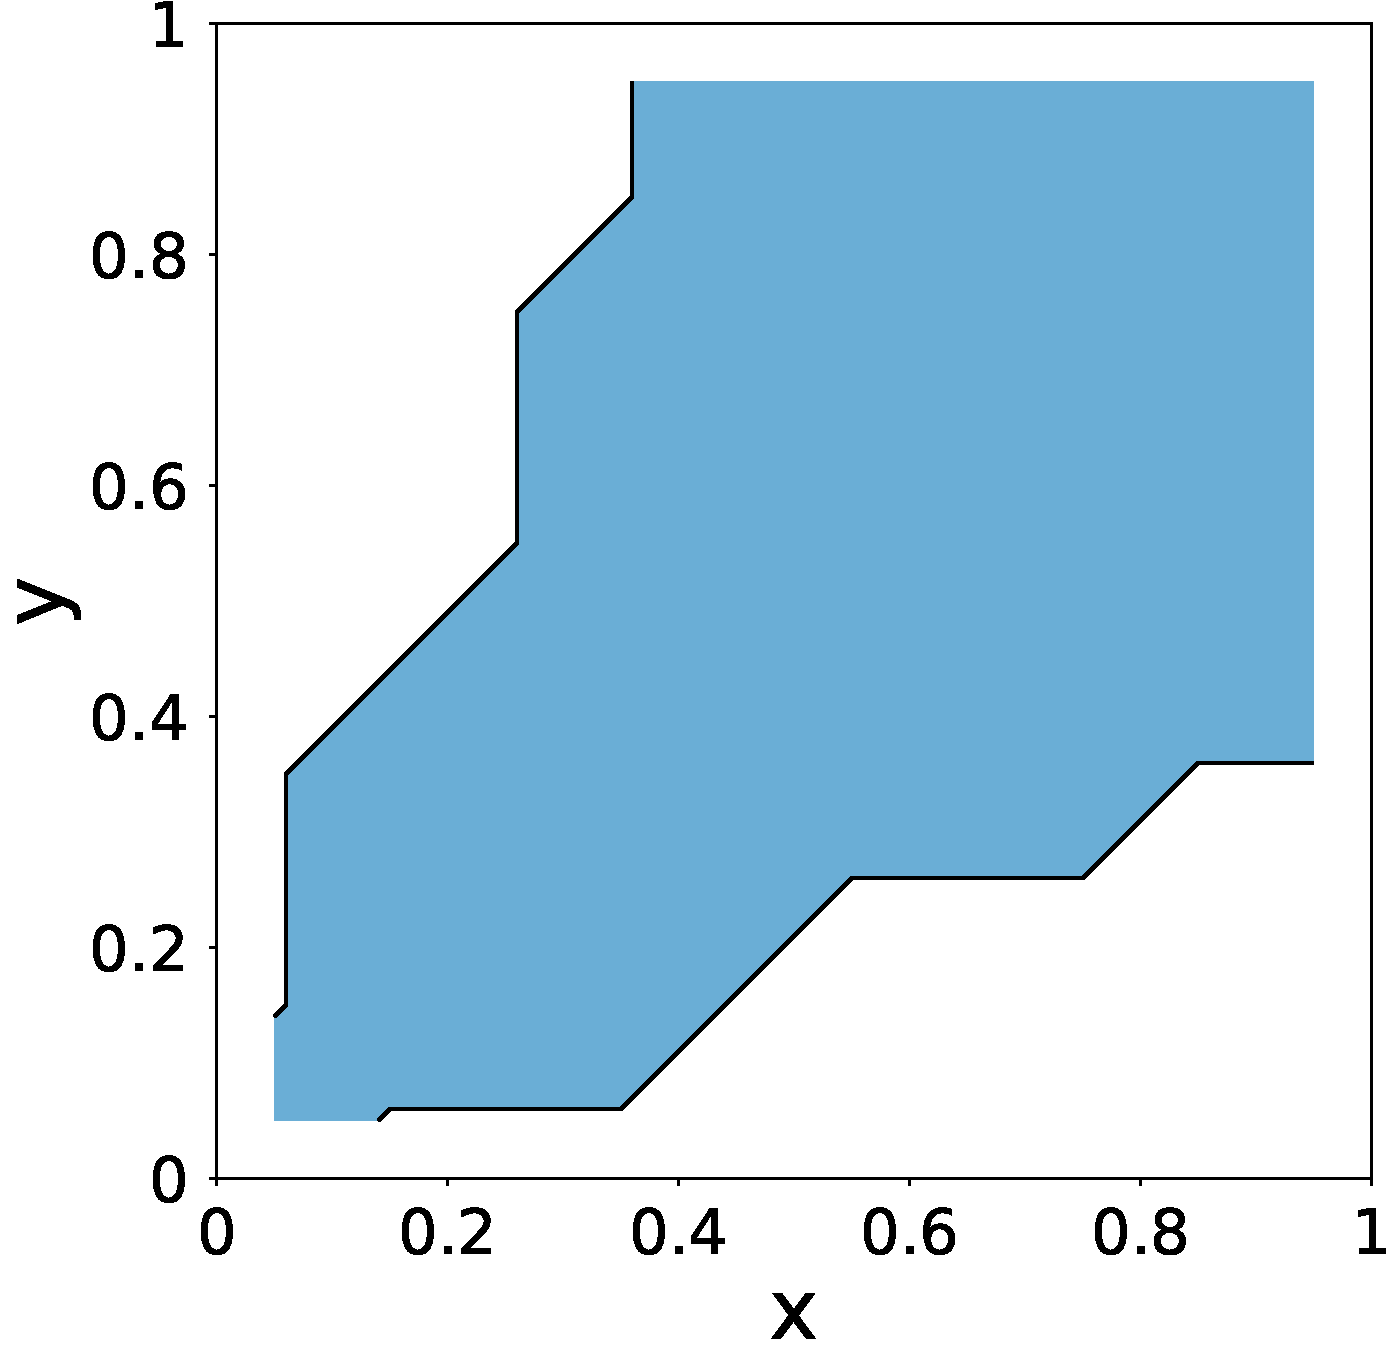
\includegraphics[scale=\smallScl]{fig1_1.pdf}}}\quad
	\subfloat{\stackinset{c}{}{t}{-.2in}{$\bm{n=50}$}{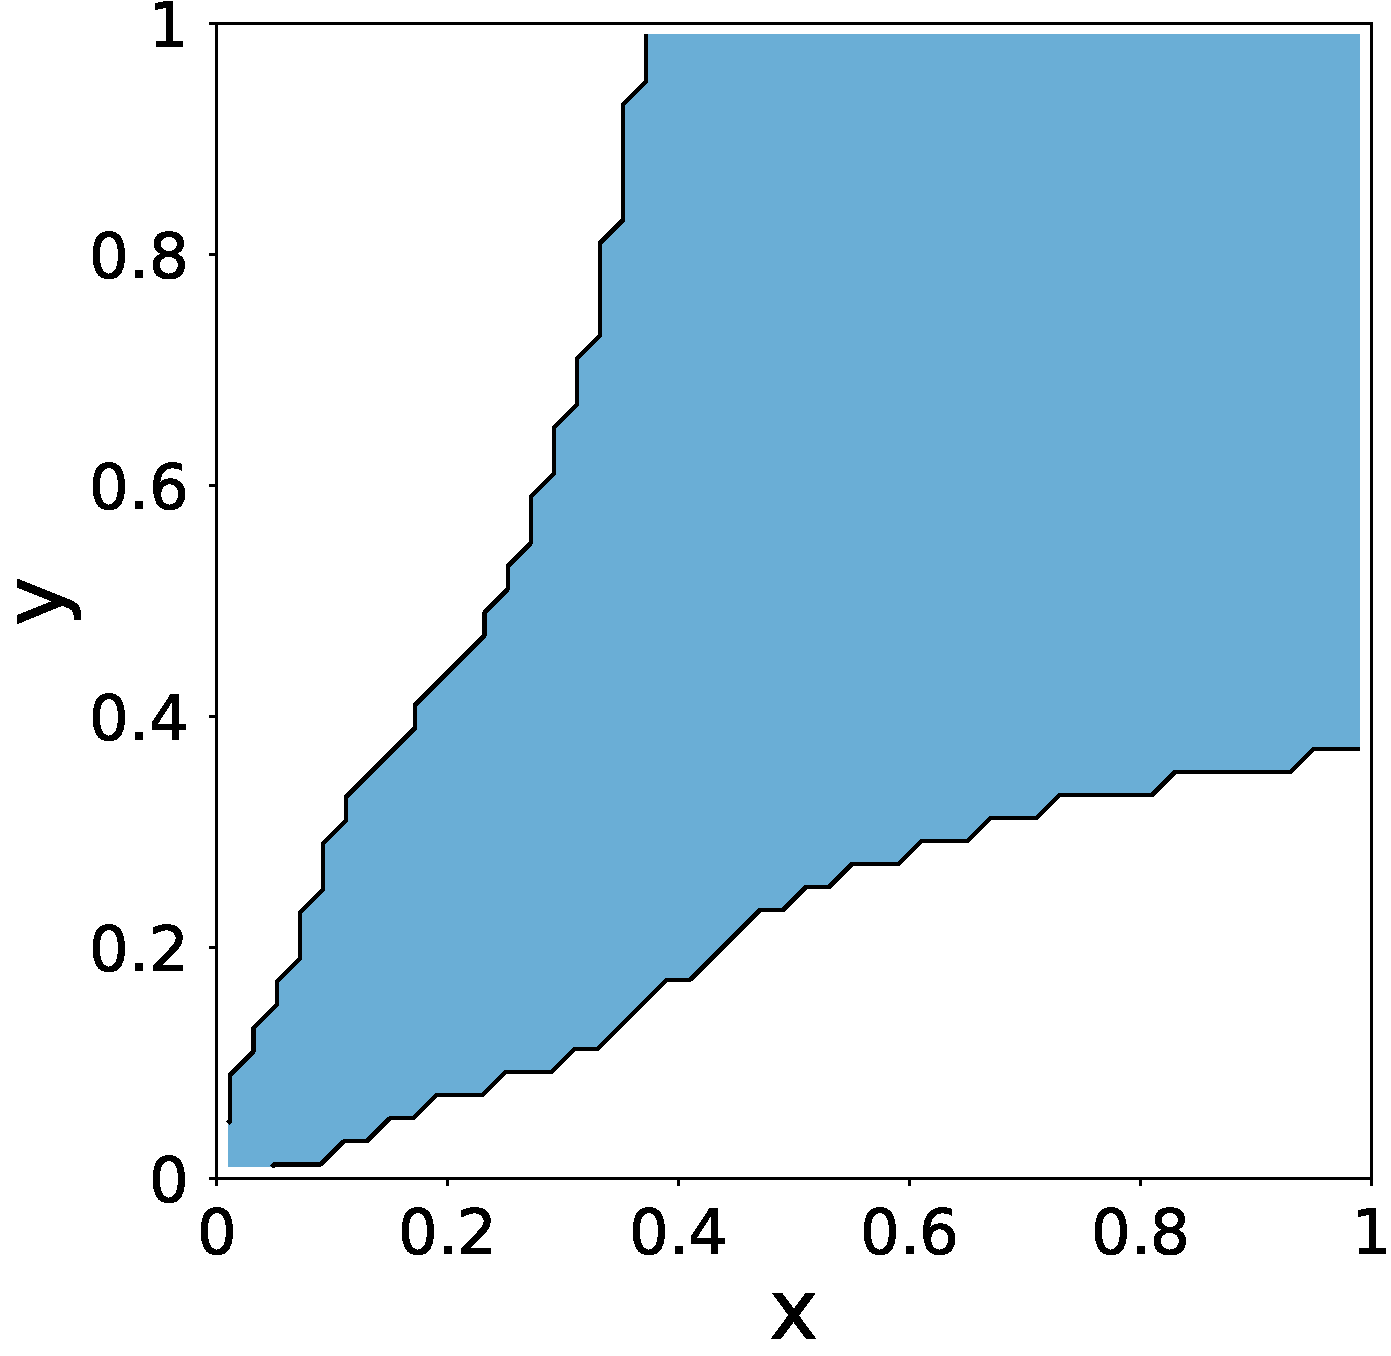
\includegraphics[scale=\smallScl]{fig1_2.pdf}}}\quad
	\subfloat{\stackinset{c}{}{t}{-.2in}{$\bm{n=100}$}{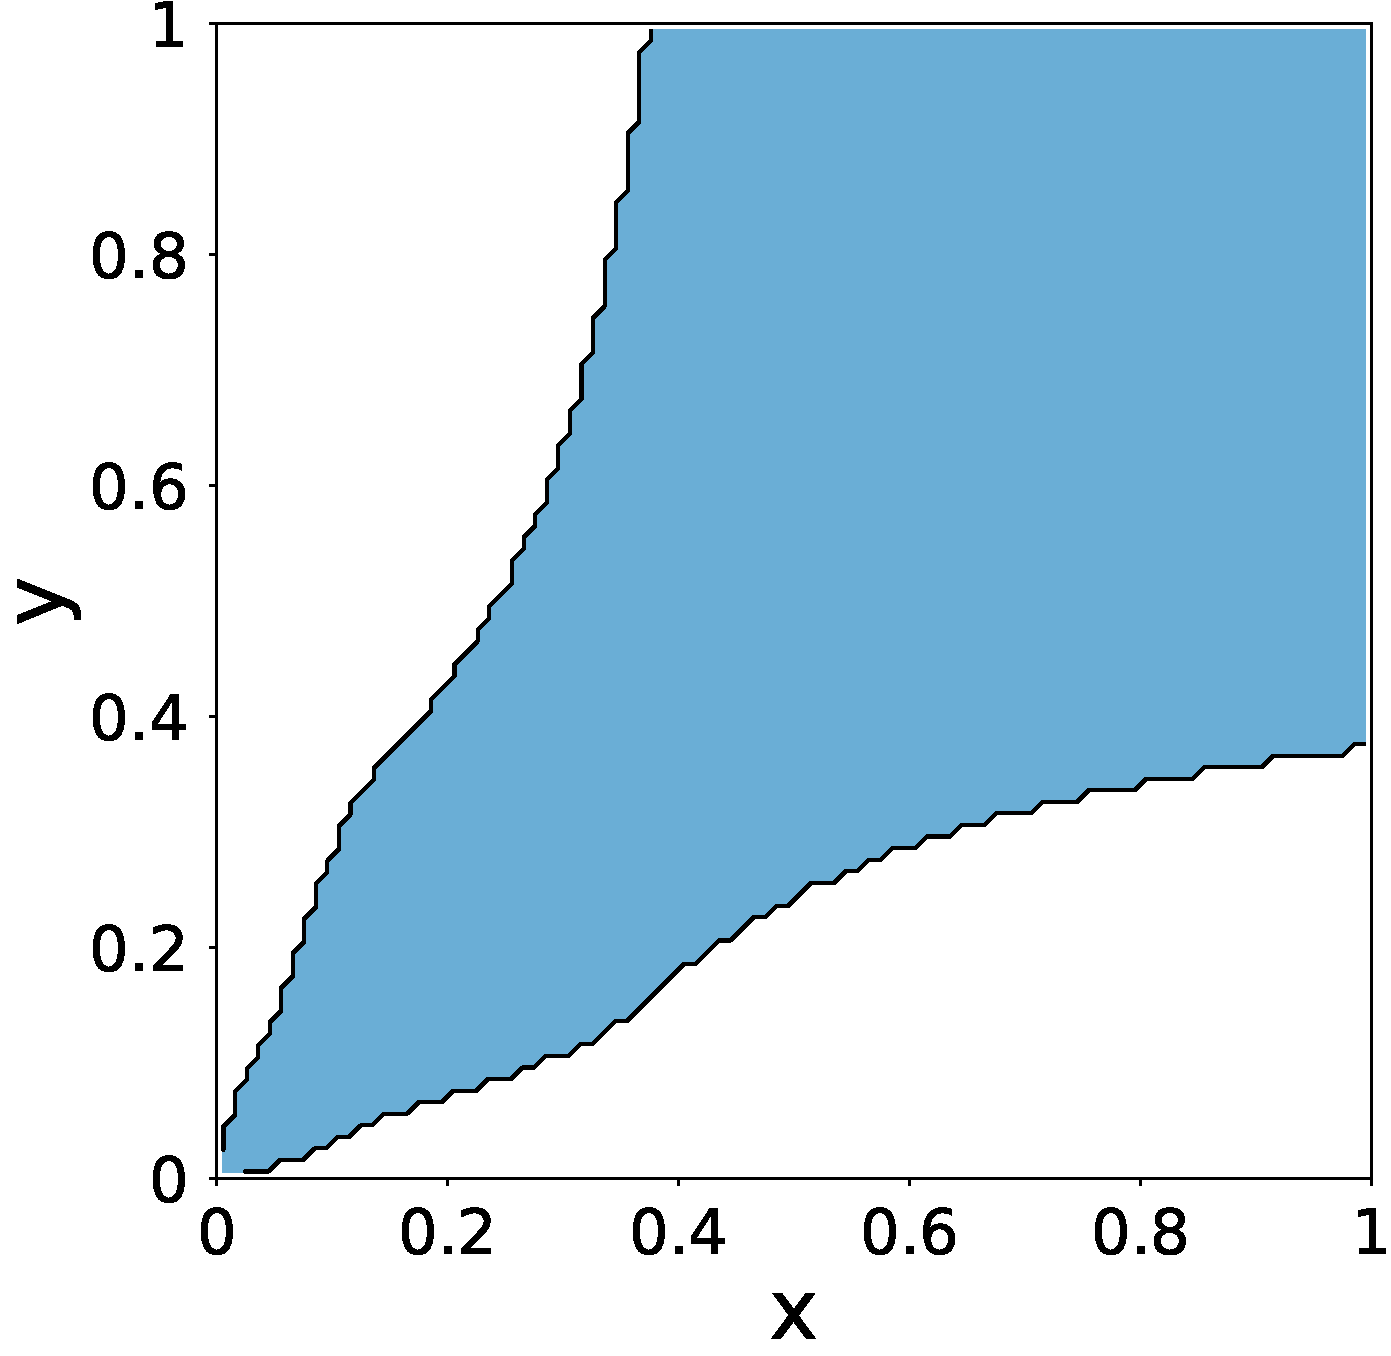
\includegraphics[scale=\smallScl]{fig1_3.pdf}}}\\
	\subfloat{\stackinset{c}{}{t}{-.2in}{$\bm{n=500}$}{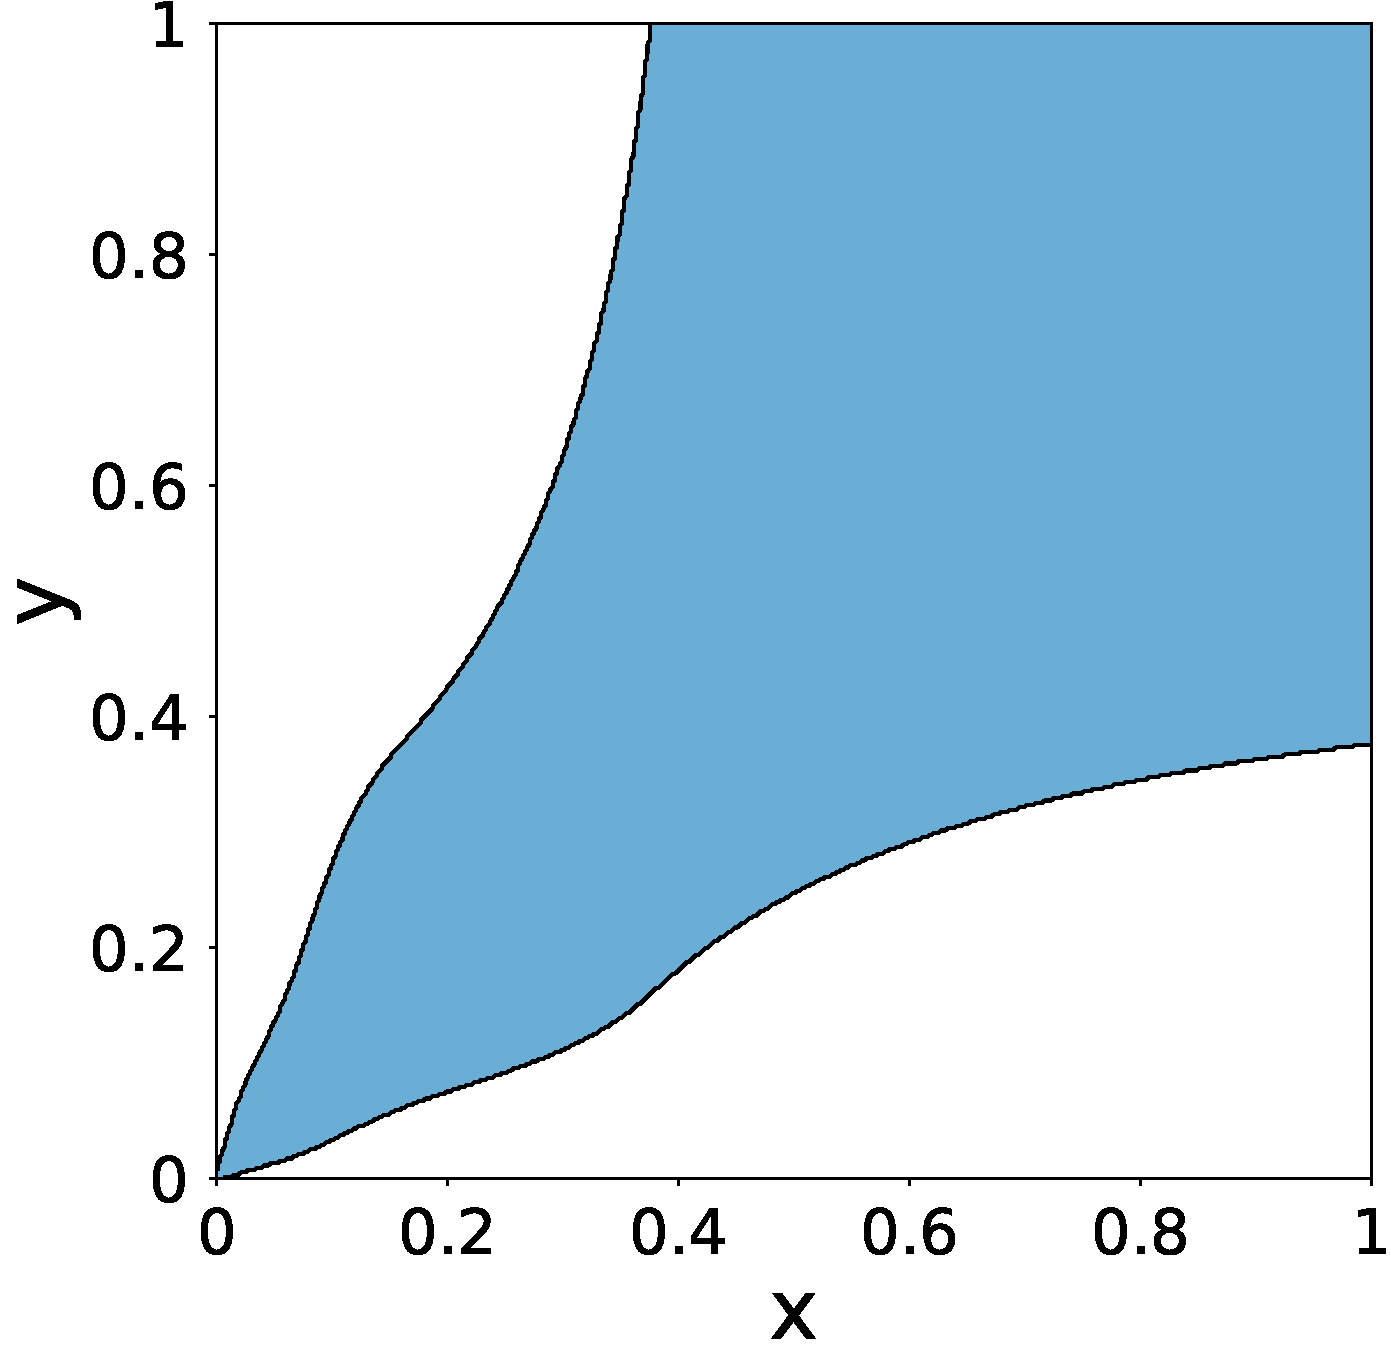
\includegraphics[scale=\largeScl]{fig1_4.pdf}}}
	\caption{Matching set at the equilibrium for several values of $n$. The points $(x,y)$ for which $\alpha(x,y)=1$ are colored in blue and the points for which $\alpha(x,y)=0$ are in white. This figure replicates figure 1 from the first reference article \citep{shimer_assortative_2000} in which utility is transferable. Parameters are $\delta=1 \ ; \ \rho=100 \ ; \ r=1 \ ; \ f(x,y)=xy \ ; \ n=500$.}
	\label{fig:fig1}
\end{figure}

 

\begin{figure}[!ht]
	\centering
	\subfloat[]{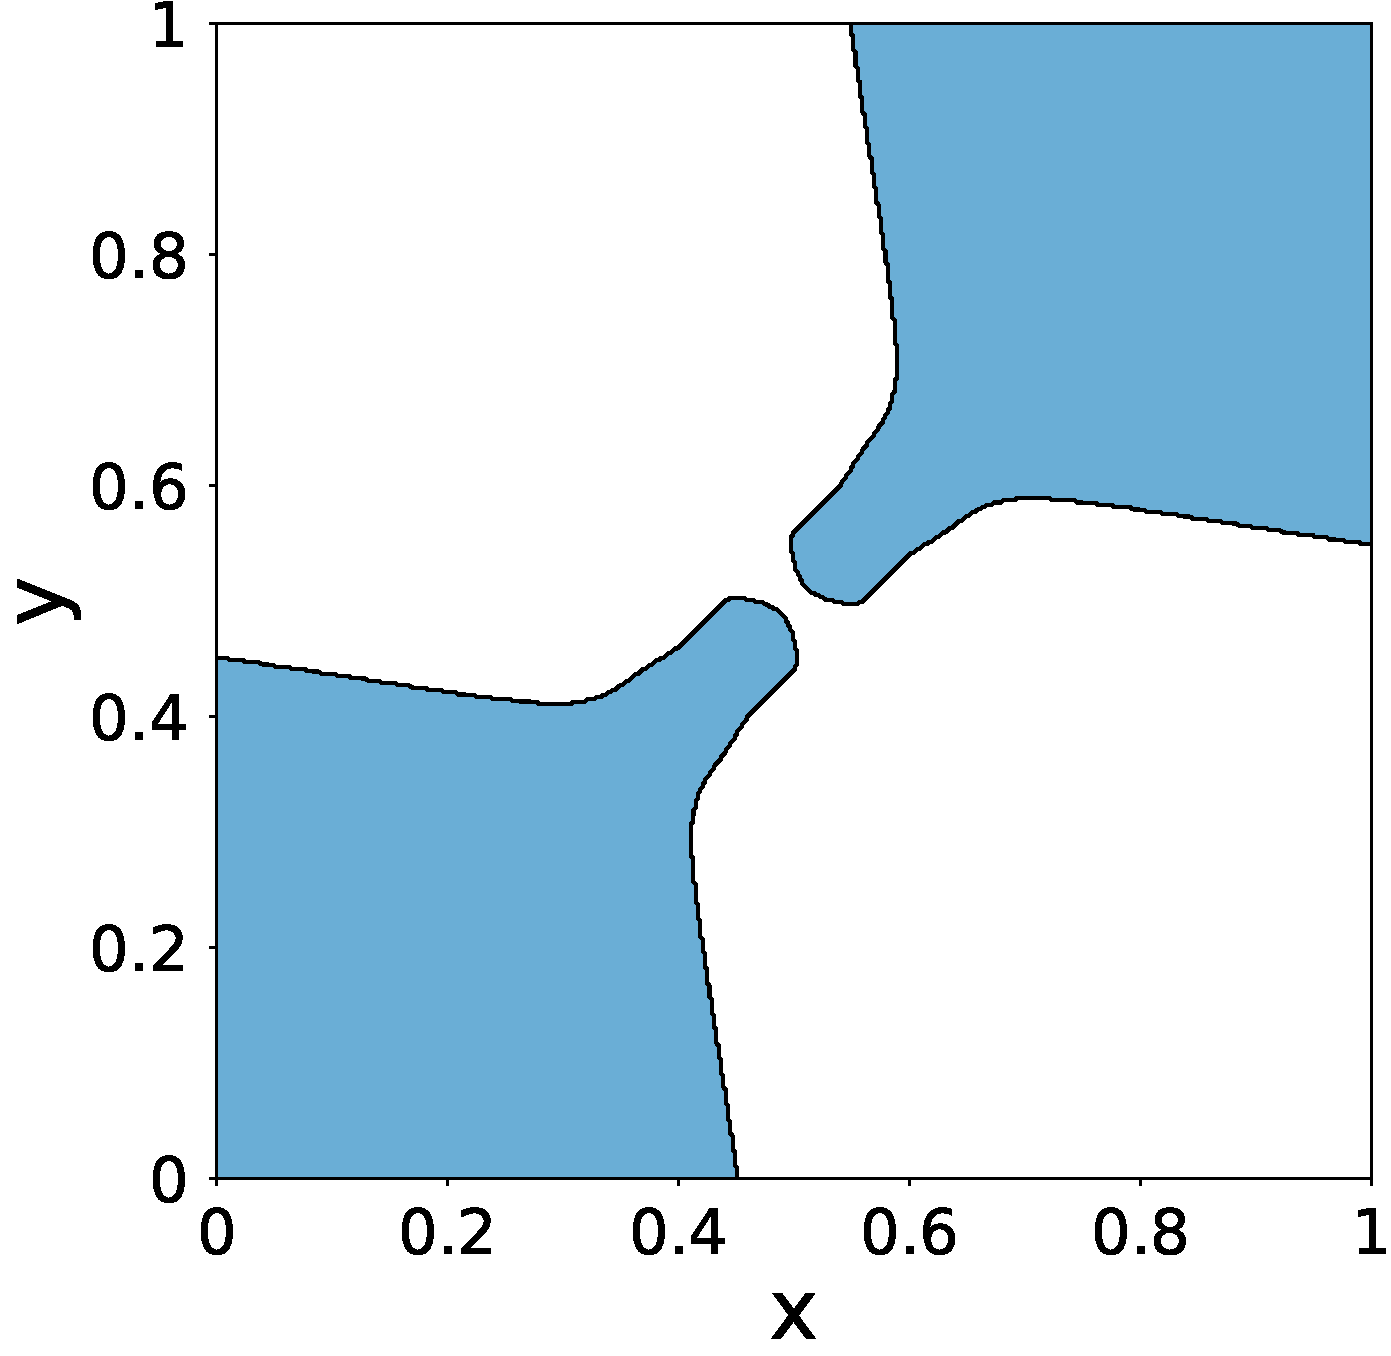
\includegraphics[scale=\mediumScl]{fig2_1.pdf}}\quad
	\subfloat[]{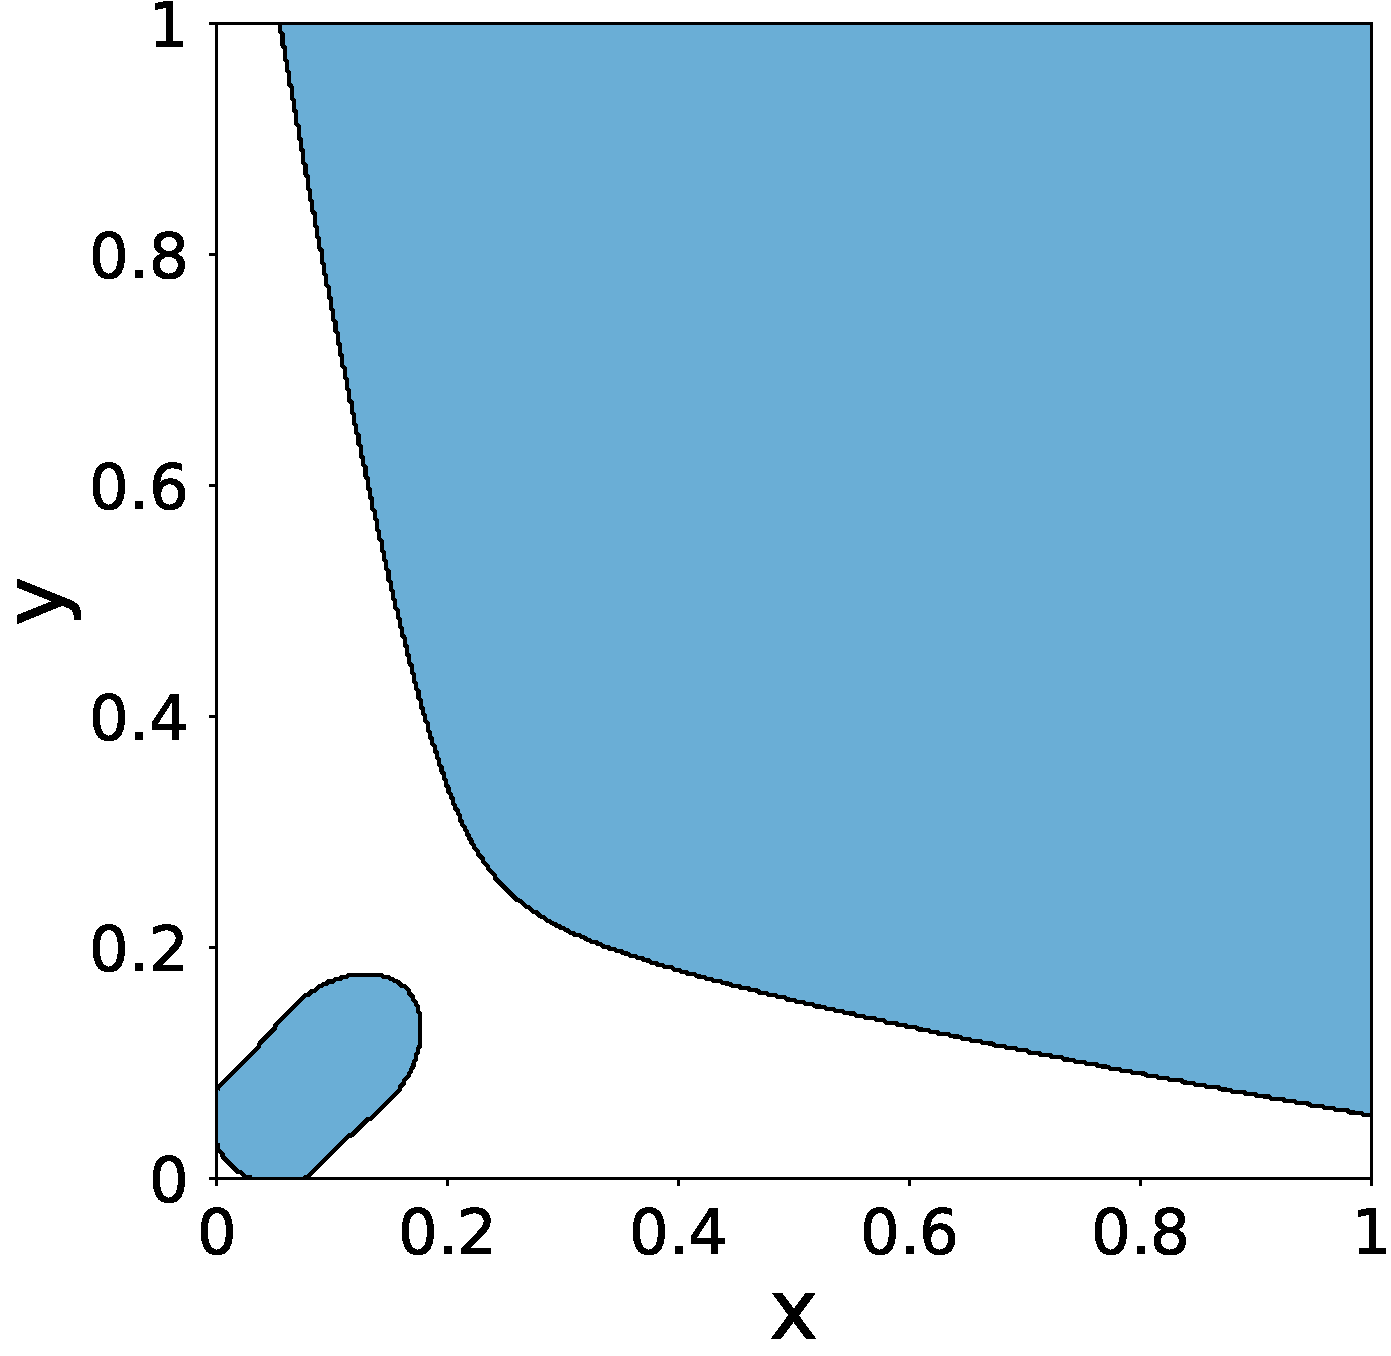
\includegraphics[scale=\mediumScl]{fig2_2.pdf}}\\
	\subfloat[]{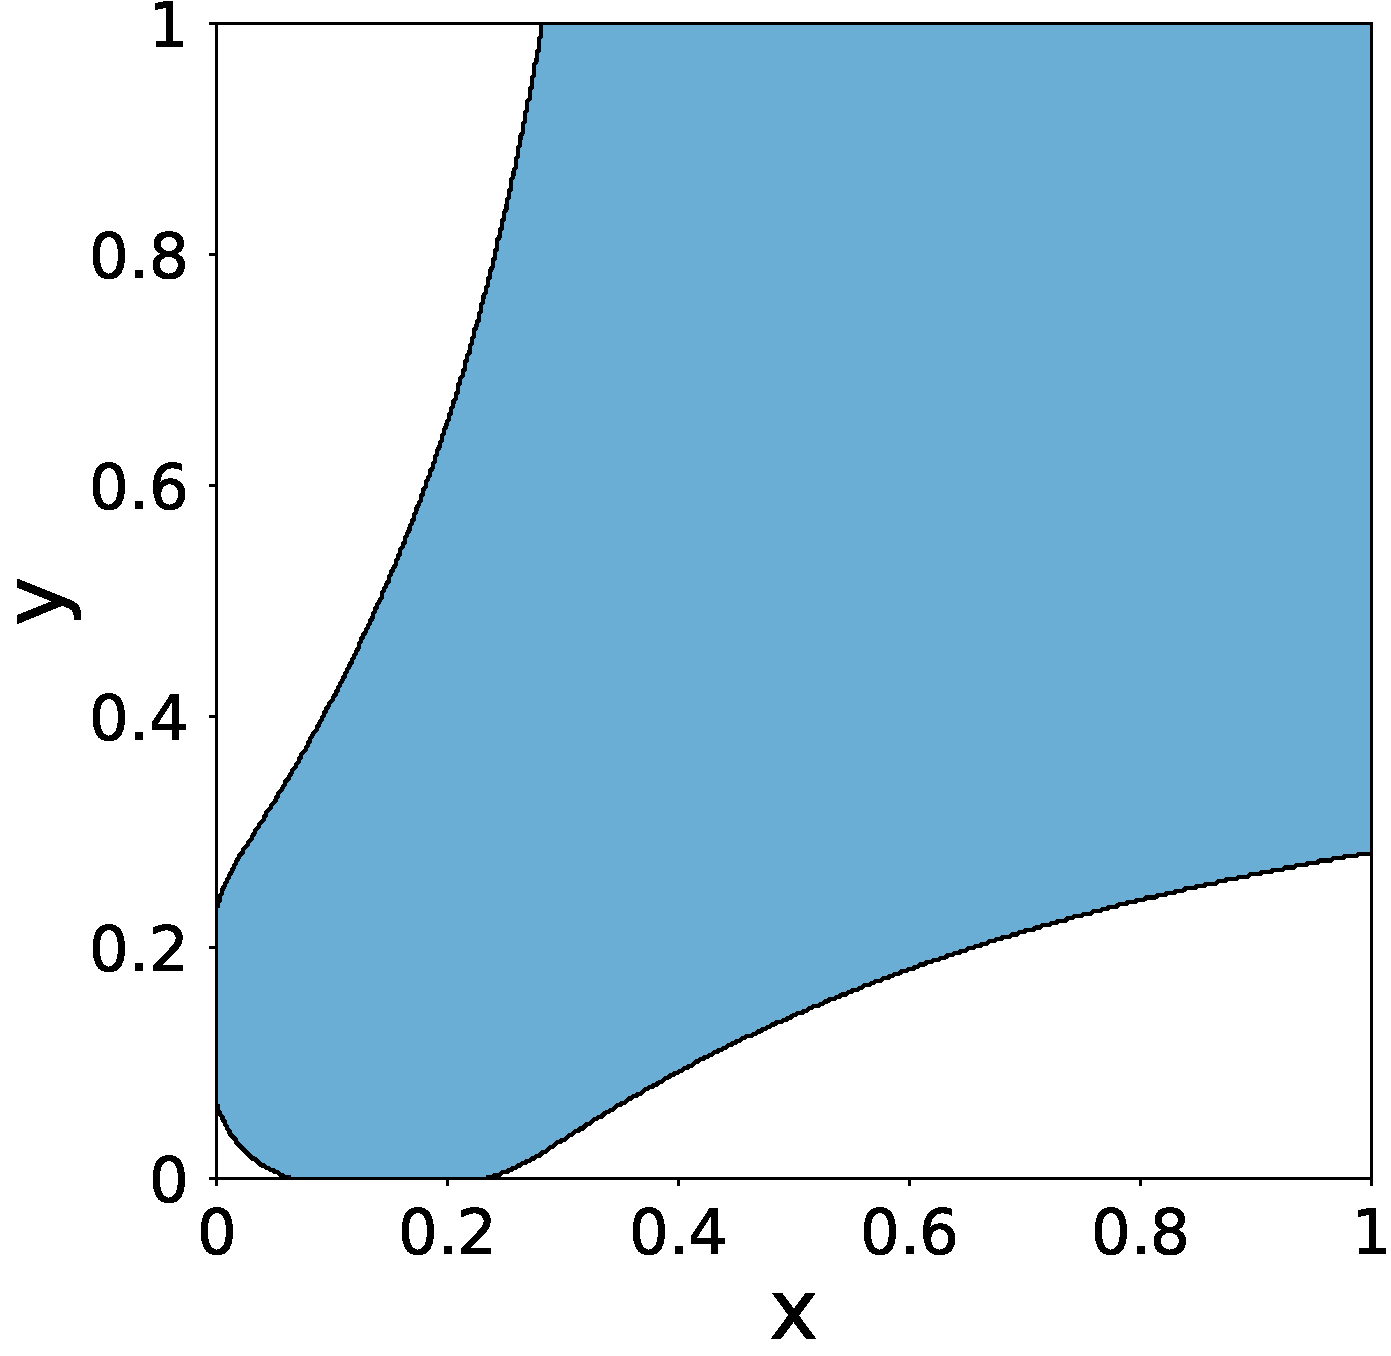
\includegraphics[scale=\mediumScl]{fig2_3.pdf}}\quad
	\subfloat[]{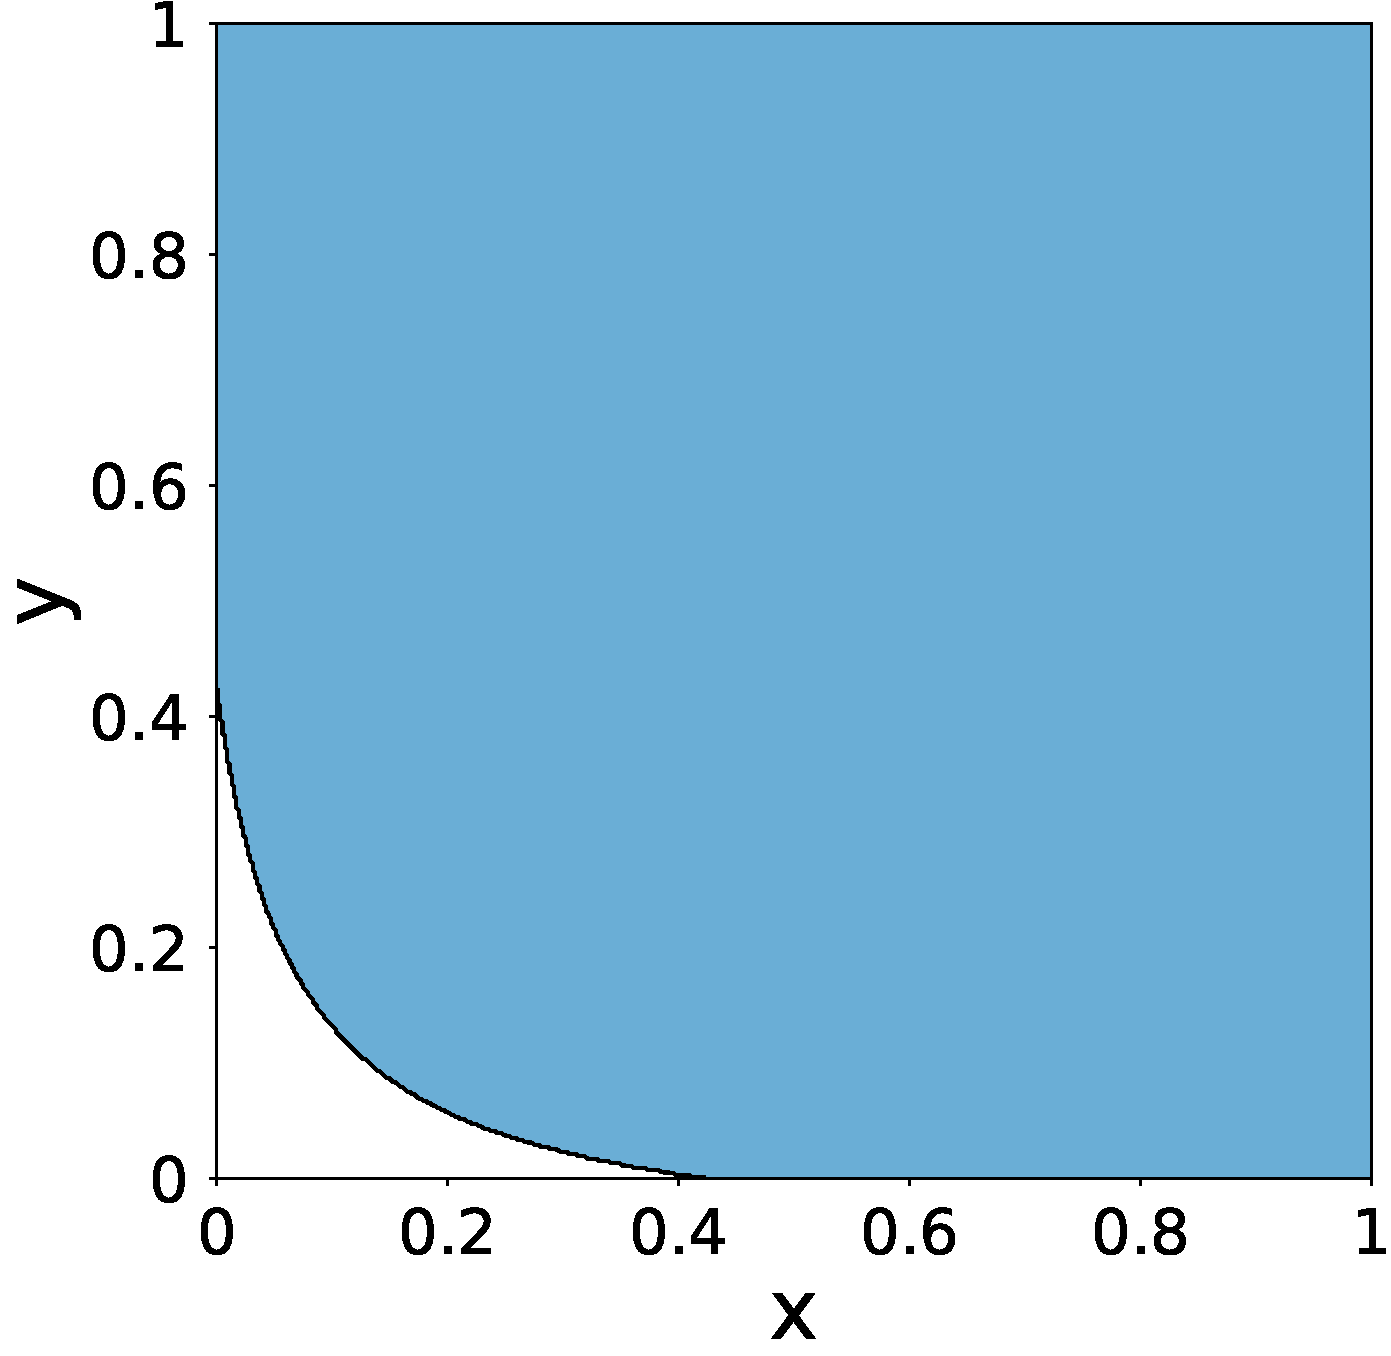
\includegraphics[scale=\mediumScl]{fig2_4.pdf}}
	\caption{Matching set at the equilibrium for transferable utility. \textbf{(A), (B)} and \textbf{(C)} respectively replicate figures 3a, 3b and figure 4 from the first reference article \citep{shimer_assortative_2000} \textbf{(D)} replicates figure 4 from \citep{smith_frictional_2011}. Parameters are \textbf{(A)} $\delta=1 \ ; \ \rho=100 \ ; \ r=1 \ ; \ f(x,y)=(x+y-1)^2$. \textbf{(B)} $\delta=1 \ ; \ \rho=35 \ ; \ r=1 \ ; \ f(x,y)=(x+y)^2 \ ; \ n=501$. \textbf{(C)} $\delta=1 \ ; \ \rho=750 \ ; \ r=1 \ ; \ f(x,y)=x+y+xy$. \textbf{(D)} $\delta=0.5 \ ; \ \rho=50 \ ; \ r=1 \ ; \ f(x,y)=x+y+xy$}
	\label{fig:fig2}
\end{figure}





\begin{figure}[!ht]
	\centering
	\subfloat[]{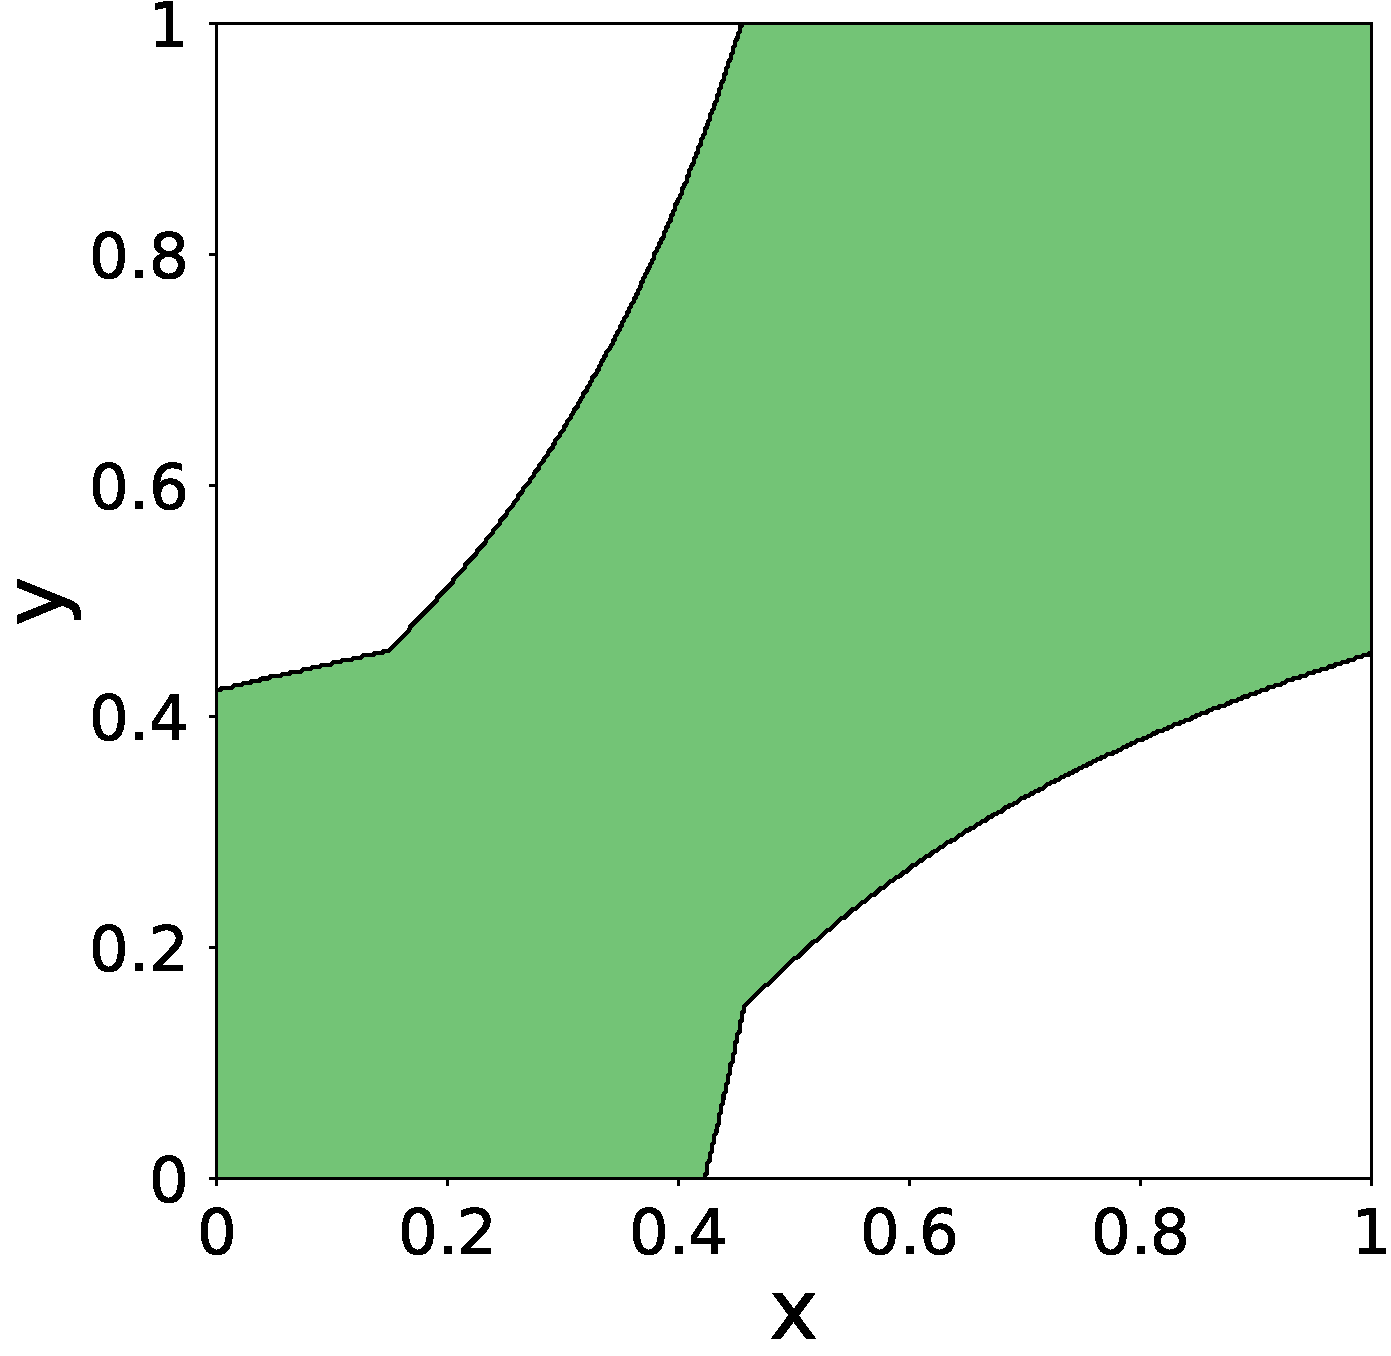
\includegraphics[scale=\mediumScl]{fig3_1.pdf}}\quad
	\subfloat[]{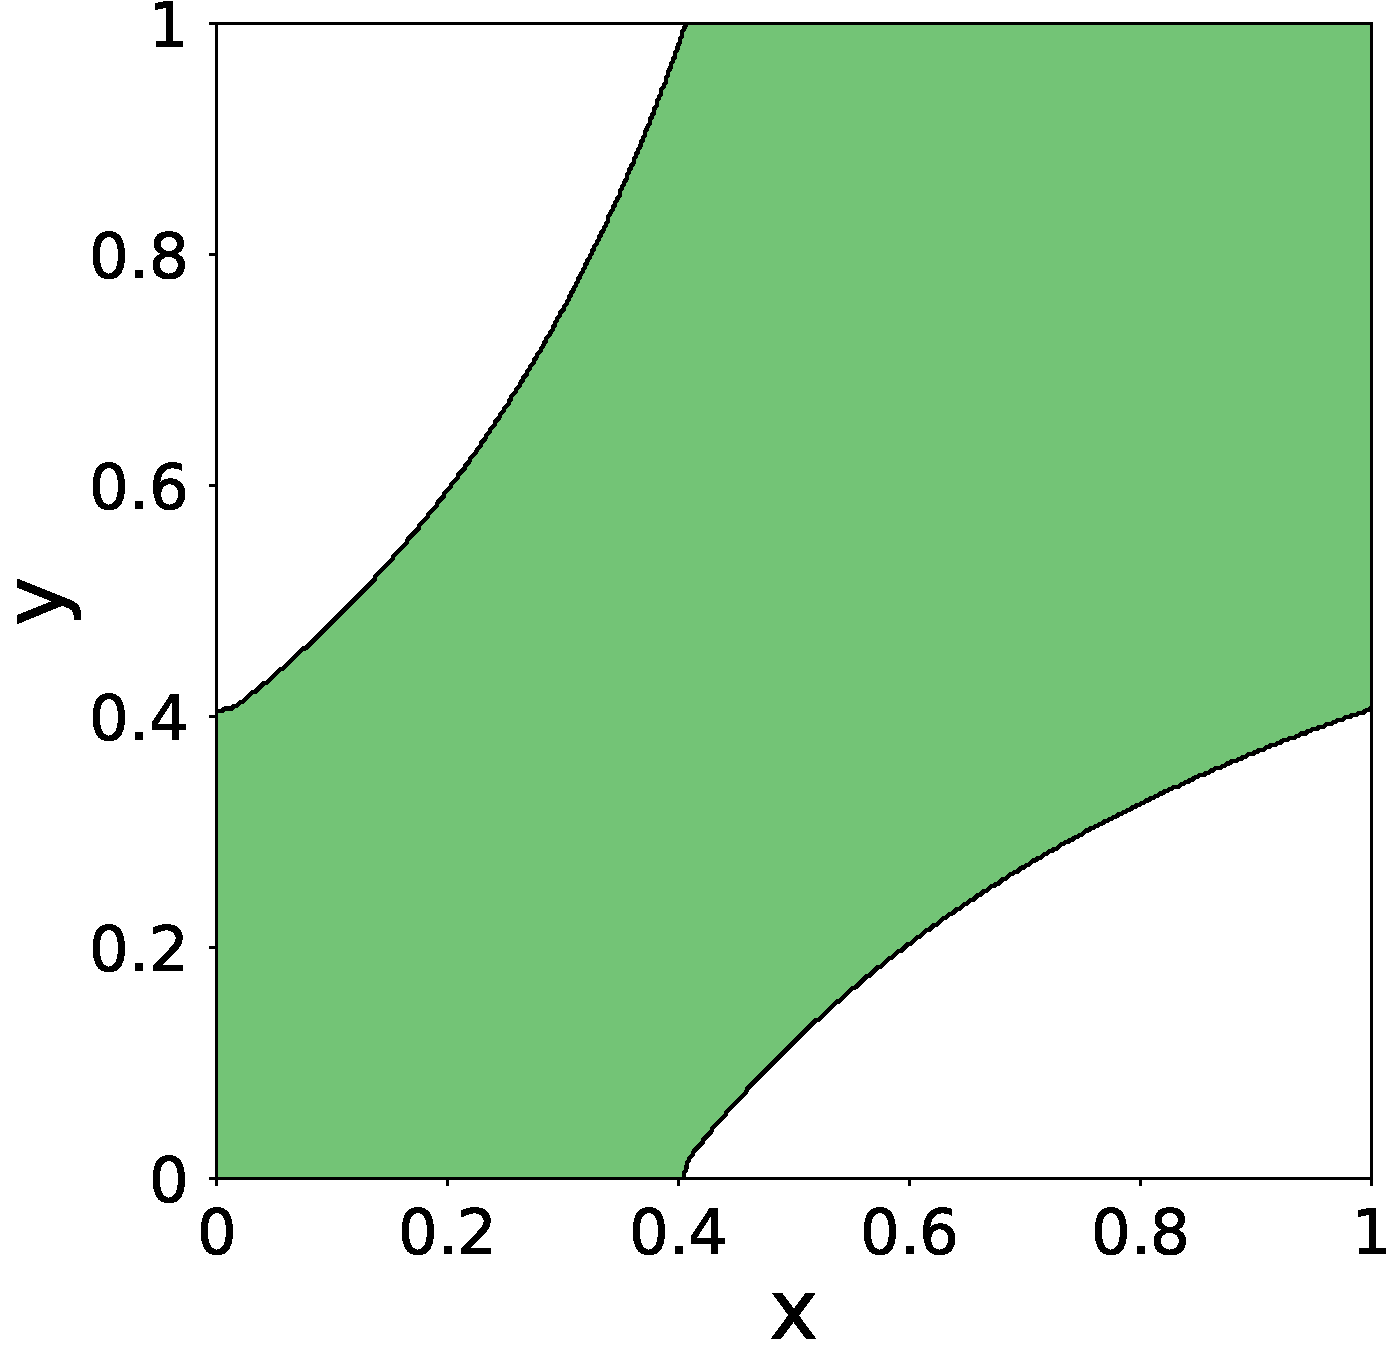
\includegraphics[scale=\mediumScl]{fig3_2.pdf}}\\
	\subfloat[]{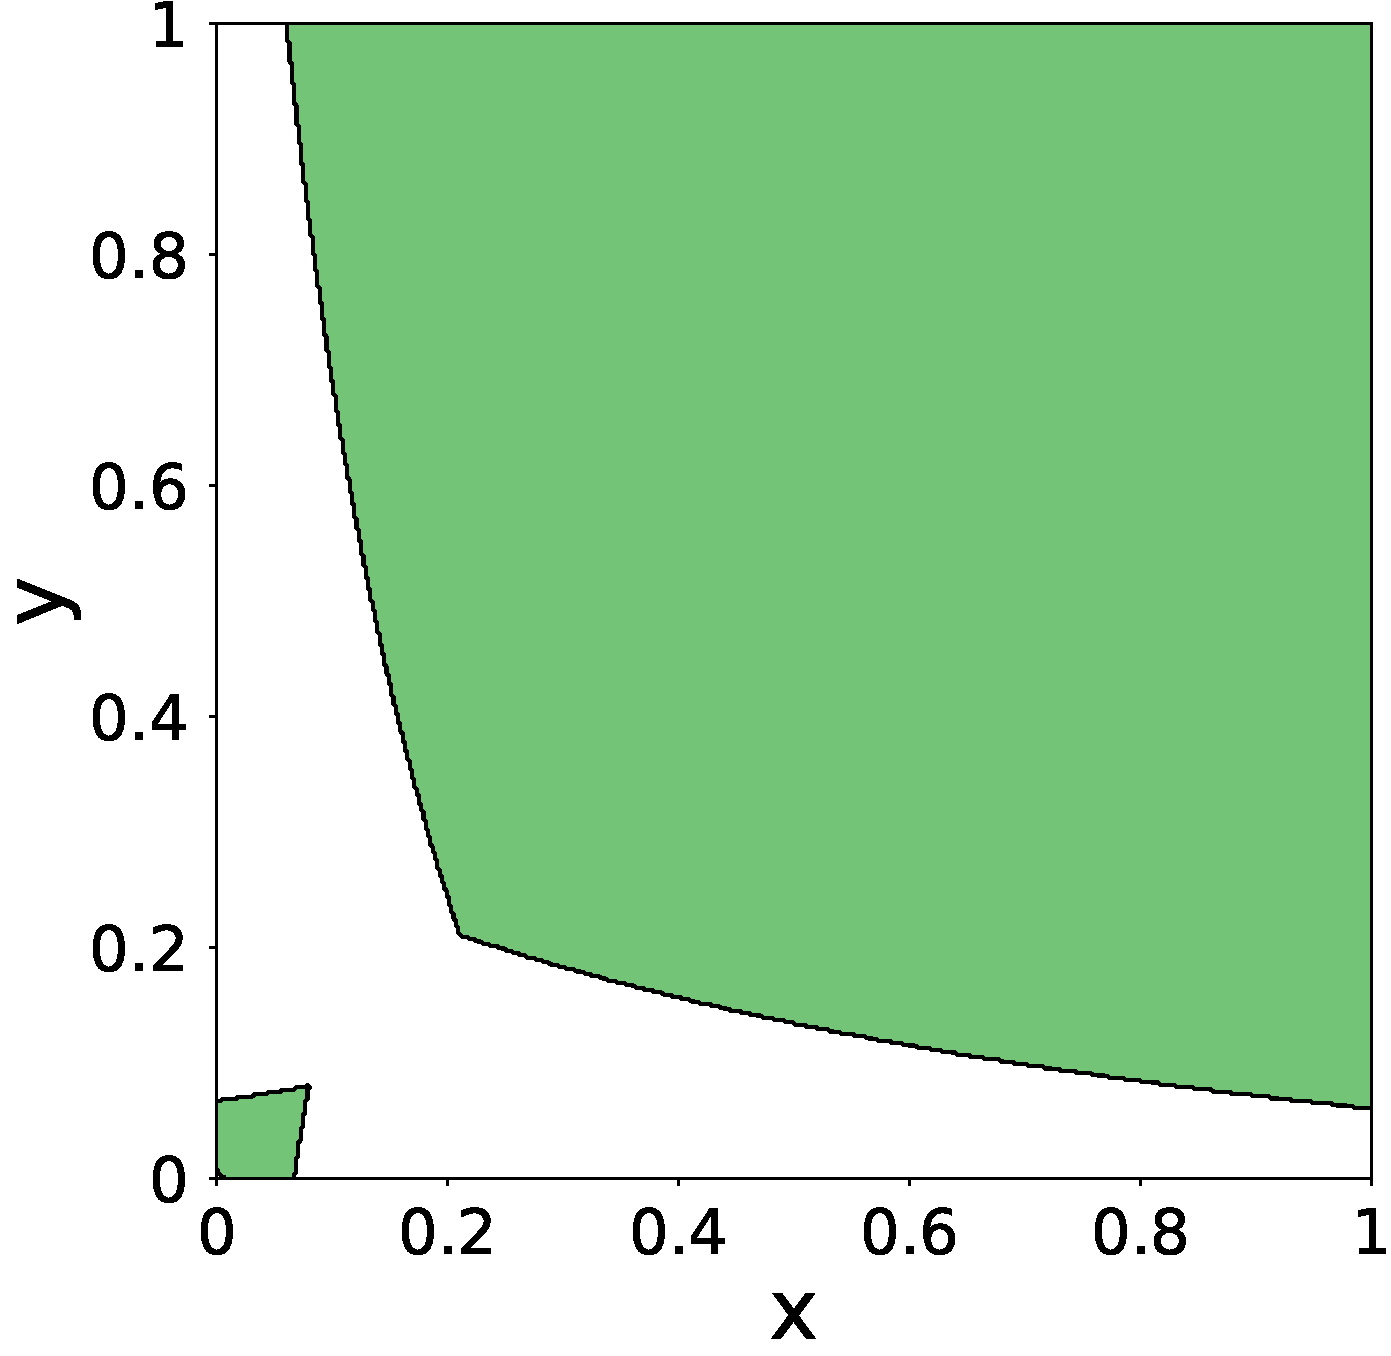
\includegraphics[scale=\mediumScl]{fig3_3.pdf}}
	\caption{Matching set at the equilibrium for non-transferable utility. \textbf{(A)} and \textbf{(B)} are attempts at replicating figure 1 from the second reference article \citep{smith_marriage_2006}. \textbf{(C)} replicates figure 2 from \citep{smith_marriage_2006}. Parameters are \textbf{(A)} $\delta=0.1 \ ; \ \rho=30 \ ; \ r=0.3 \ ; \ f(x,y)=e^{xy}$. \textbf{(B)} $\delta=0.1 \ ; \ \rho=30 \ ; \ r=0.3 \ ; \ f(x,y)=e^{xy}$. \textbf{(C)} $\delta=0.1 \ ; \ \rho=3 \ ; \ r=0.3 \ ; \ f(x,y)=x+y+xy$.}
	\label{fig:fig3}
\end{figure}
 




\begin{figure}[!ht]
	\centering
	\raisebox{-2.5cm}{\rotatebox[origin=c]{90}{$\bm{\sigma=0.01}$}}\quad
	\subfloat{\stackinset{c}{}{t}{-.2in}{$\bm{\mu=0.2}$}{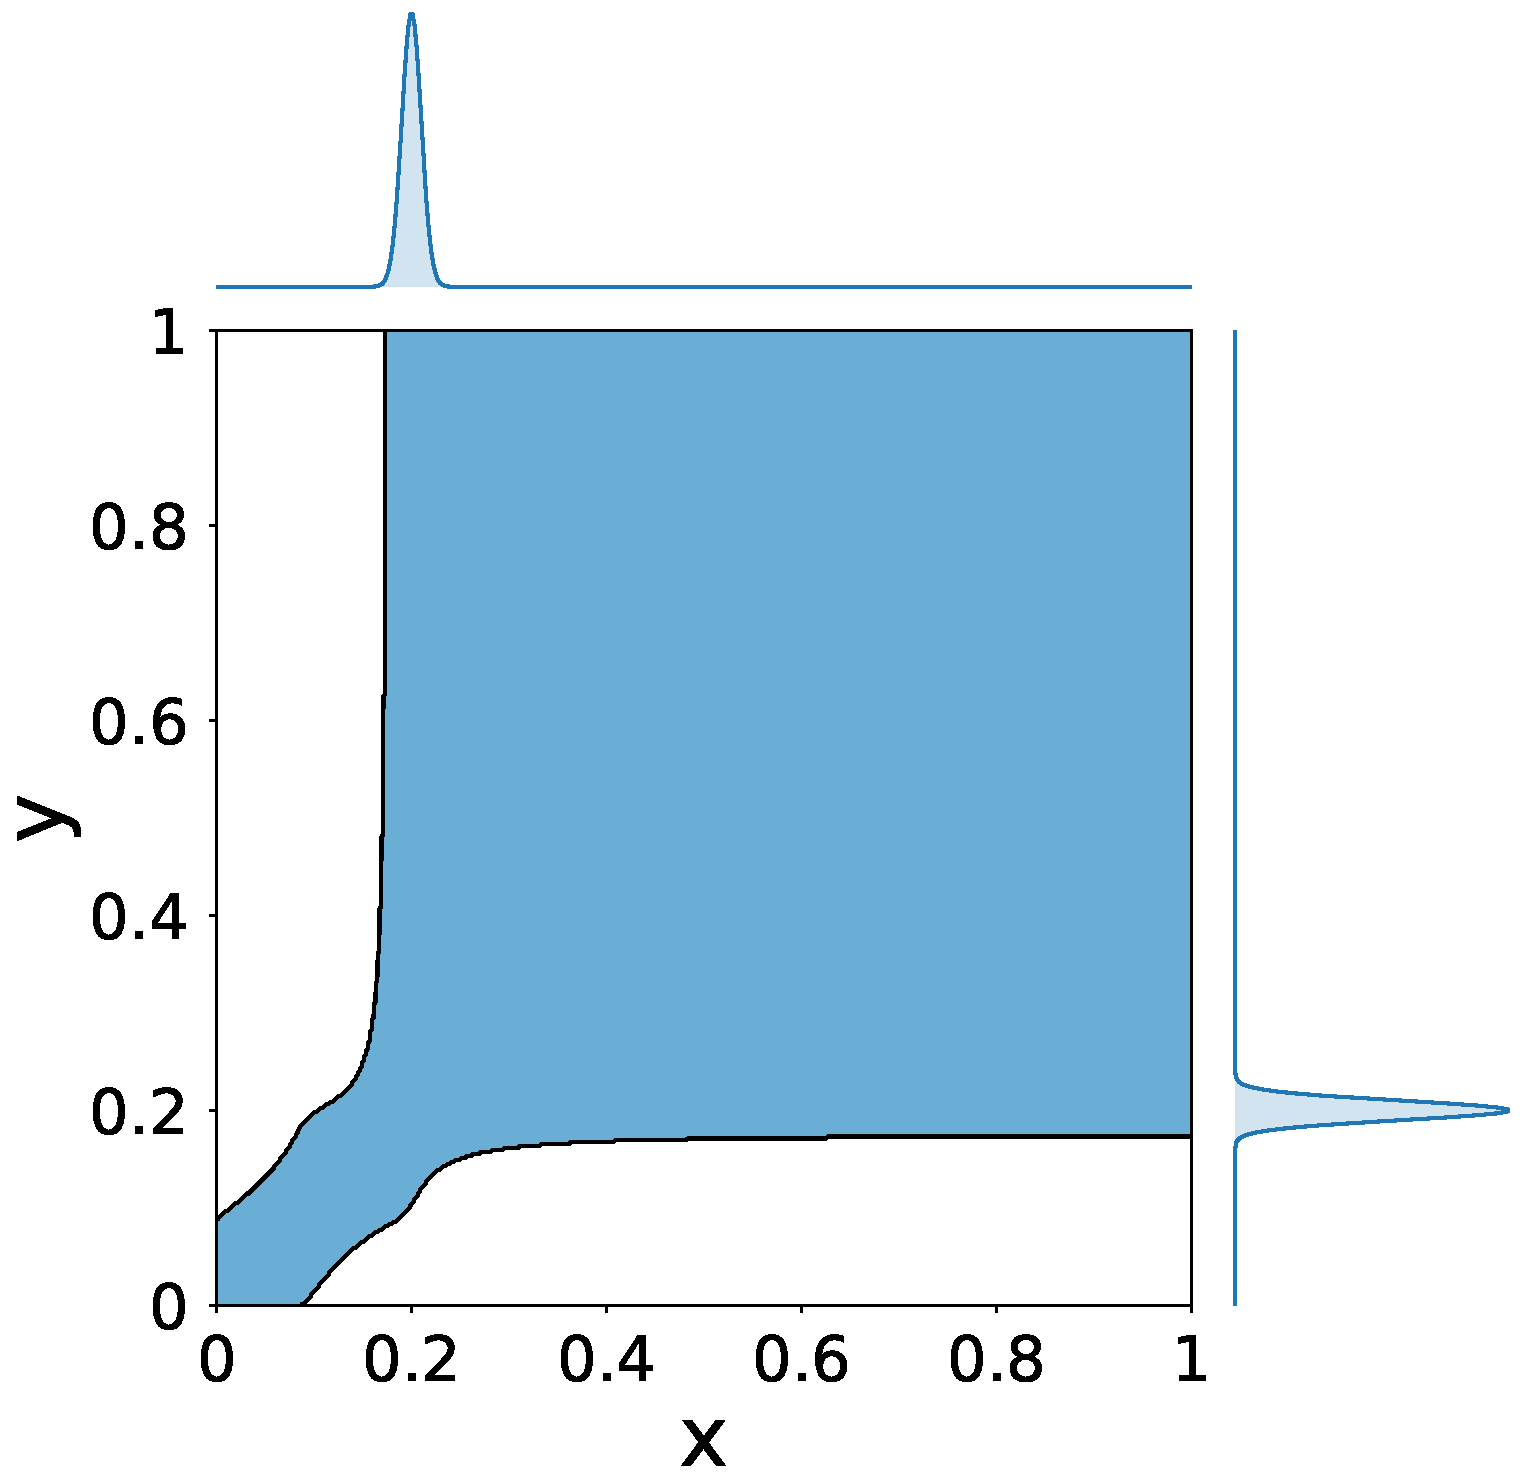
\includegraphics[scale=\smallScl]{fig4_1.pdf}}}\quad
	\subfloat{\stackinset{c}{}{t}{-.2in}{$\bm{\mu=0.5}$}{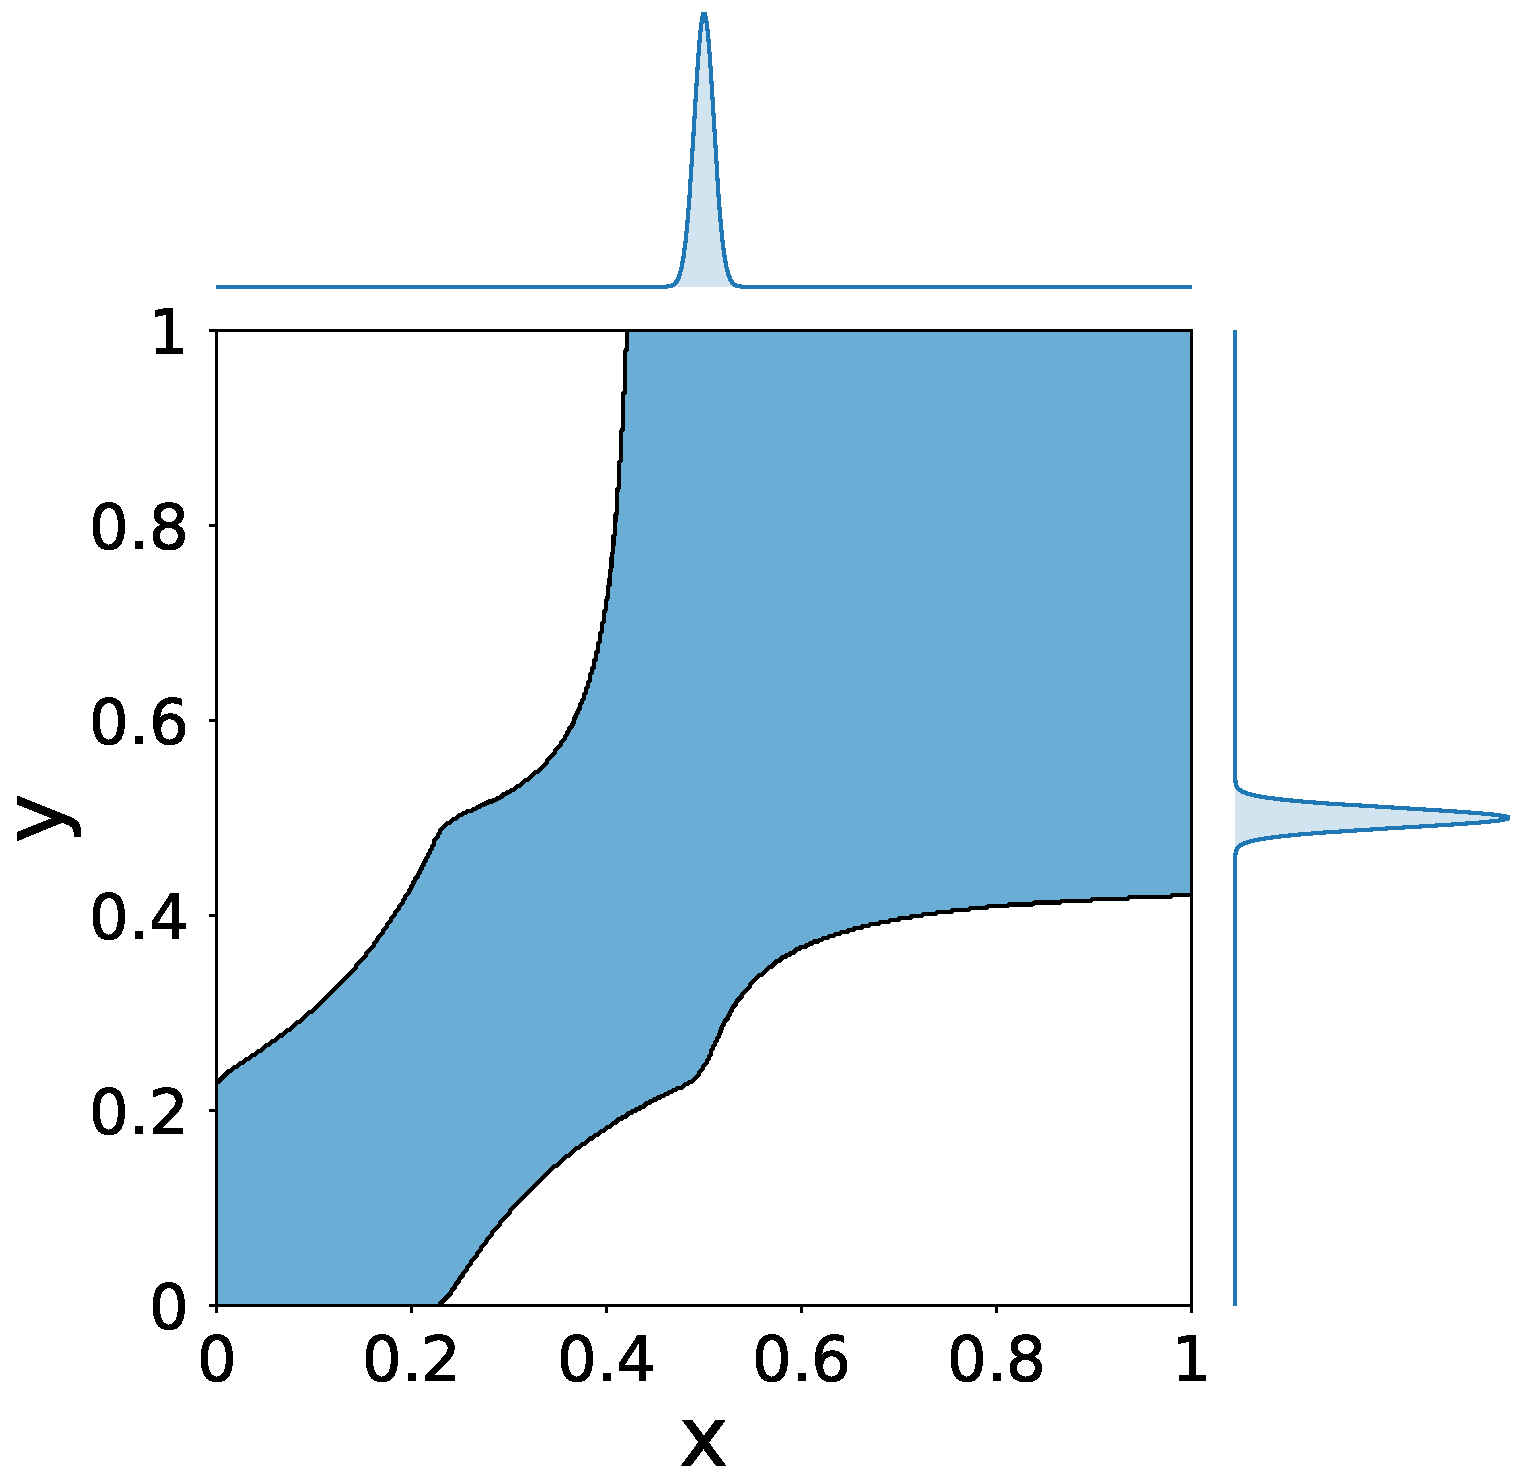
\includegraphics[scale=\smallScl]{fig4_2.pdf}}}\quad
	\subfloat{\stackinset{c}{}{t}{-.2in}{$\bm{\mu=0.8}$}{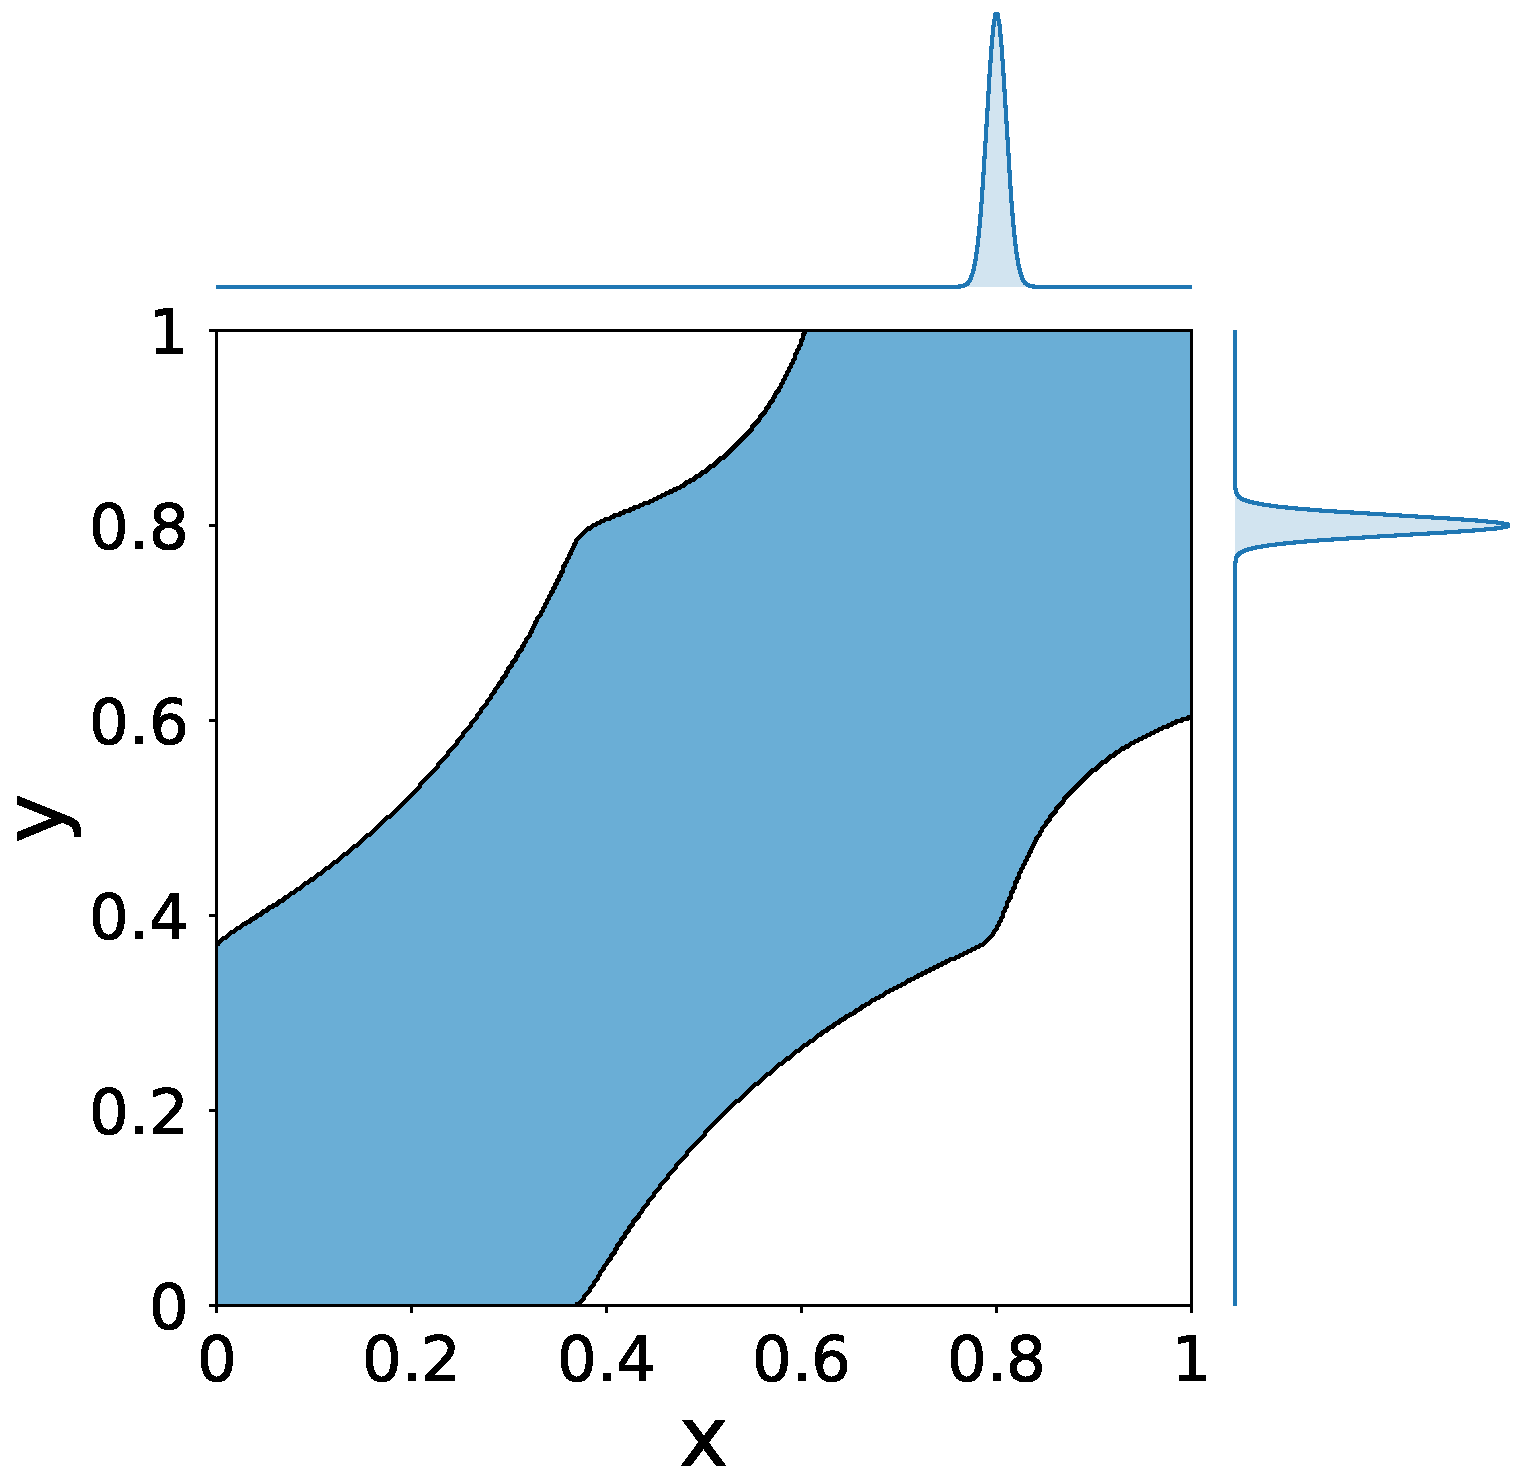
\includegraphics[scale=\smallScl]{fig4_3.pdf}}}\\
	\raisebox{-2cm}{\rotatebox[origin=c]{90}{$\bm{\sigma=0.1}$}}\quad
	\subfloat{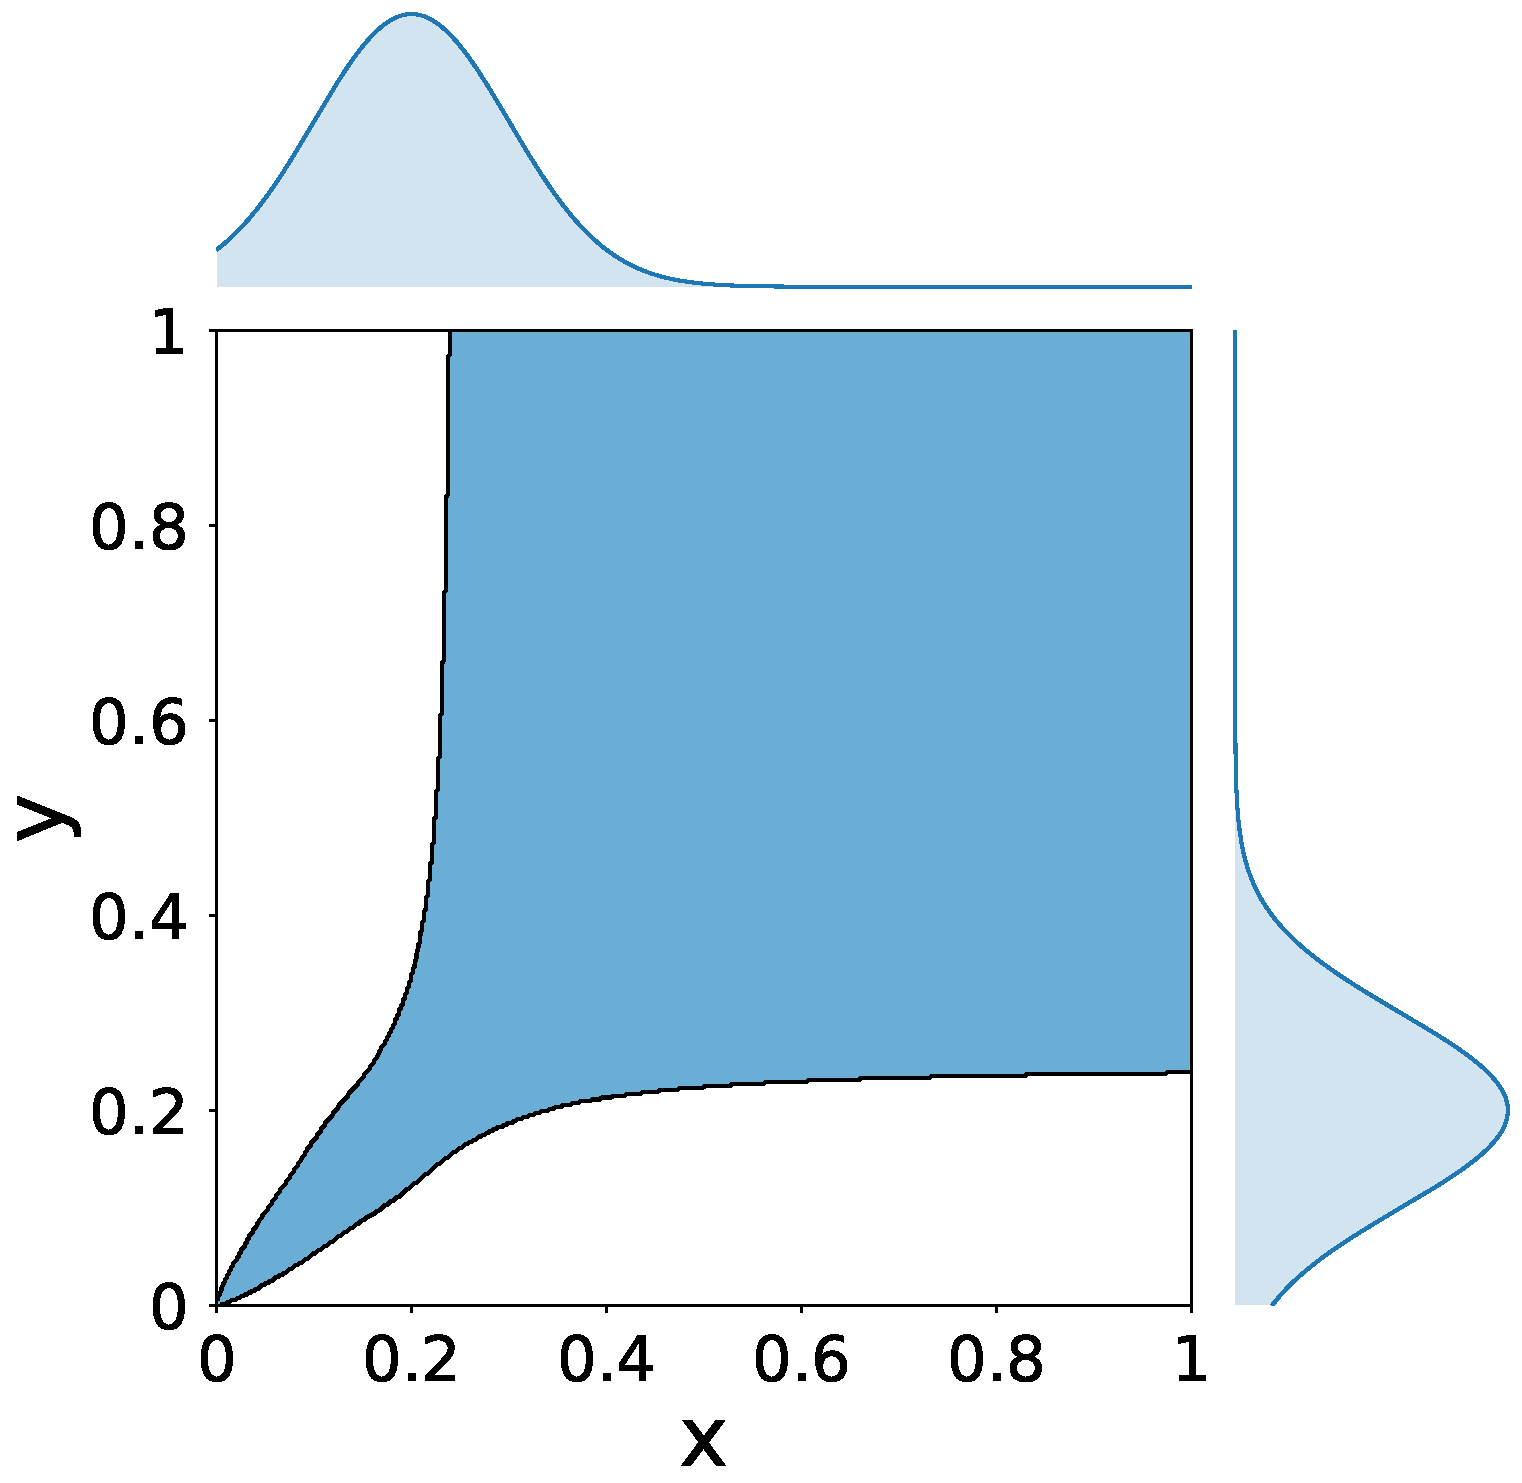
\includegraphics[scale=\smallScl]{fig4_4.pdf}}\quad
	\subfloat{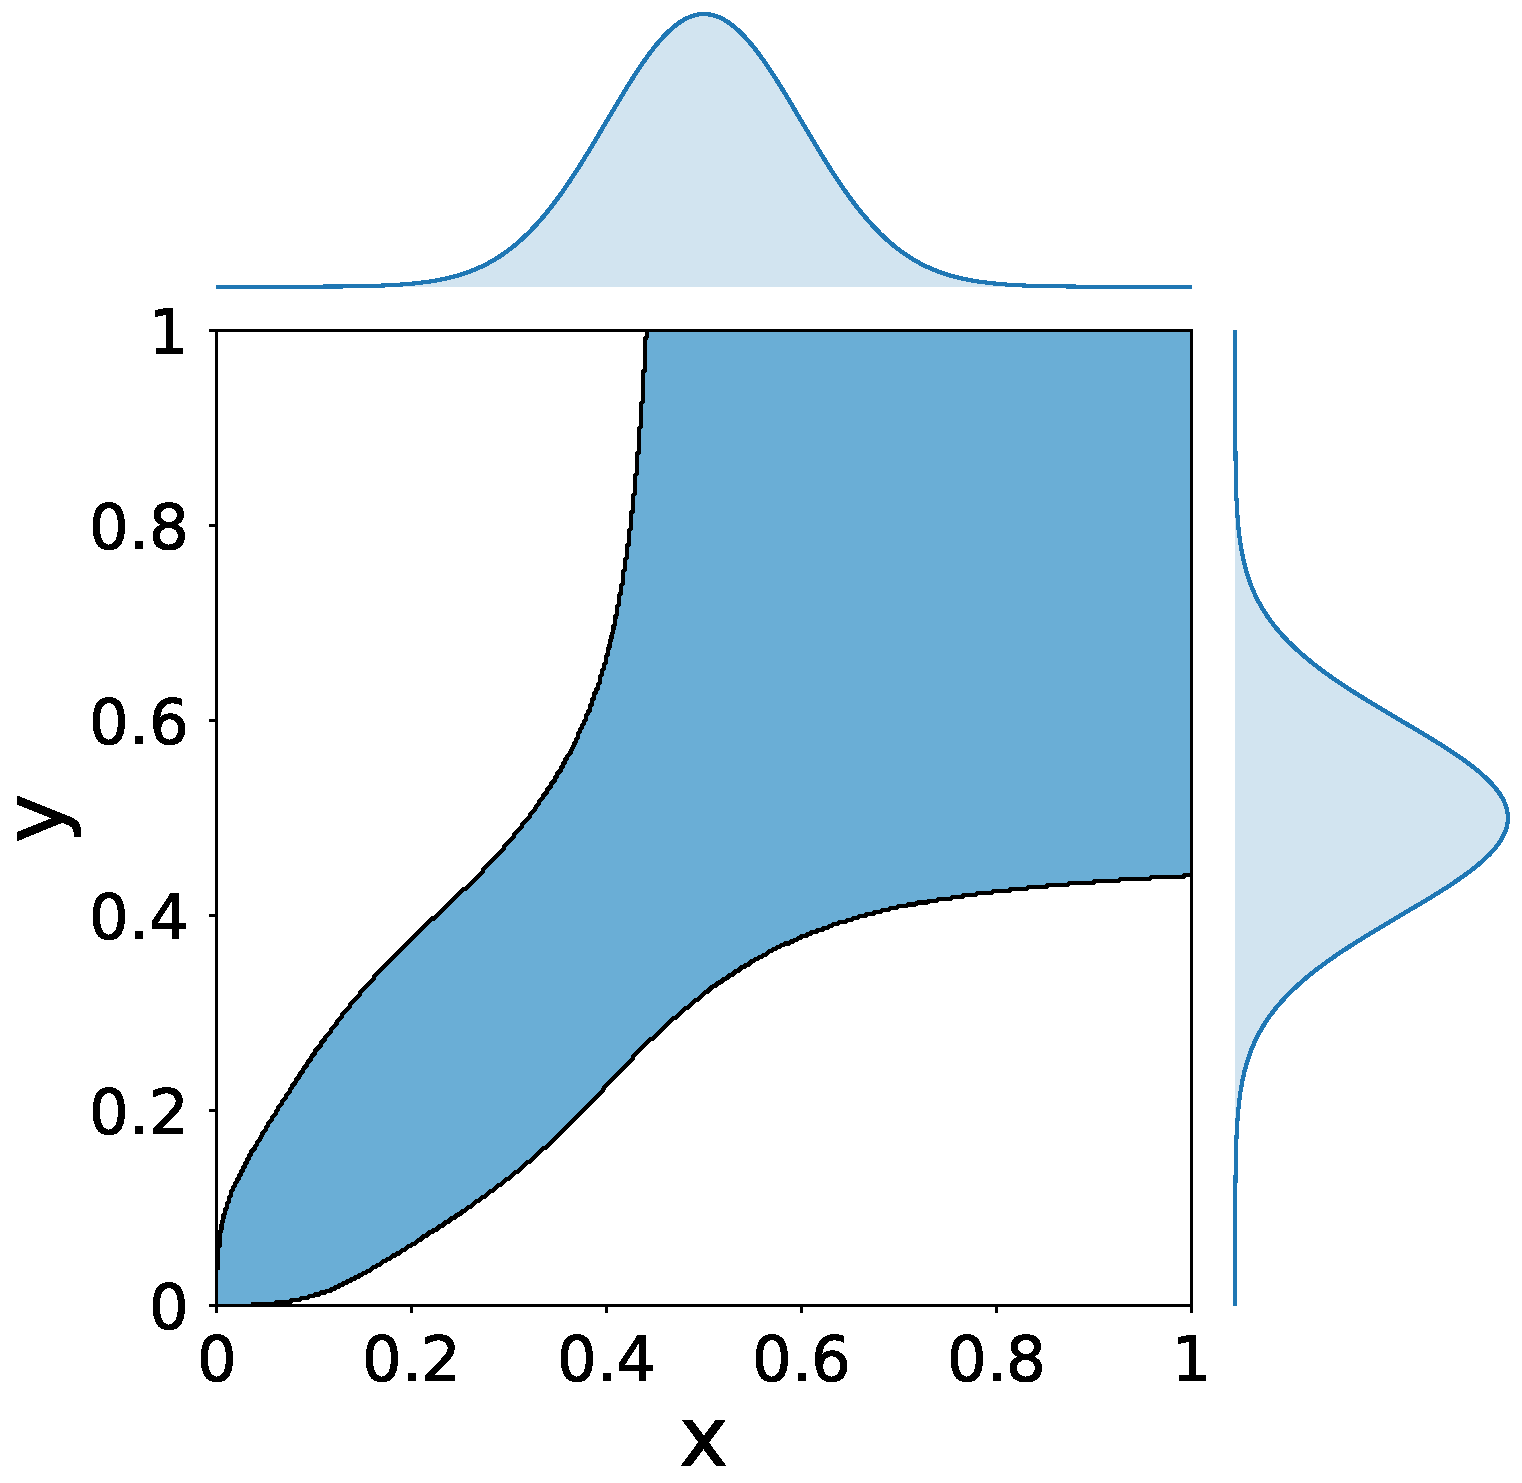
\includegraphics[scale=\smallScl]{fig4_5.pdf}}\quad
	\subfloat{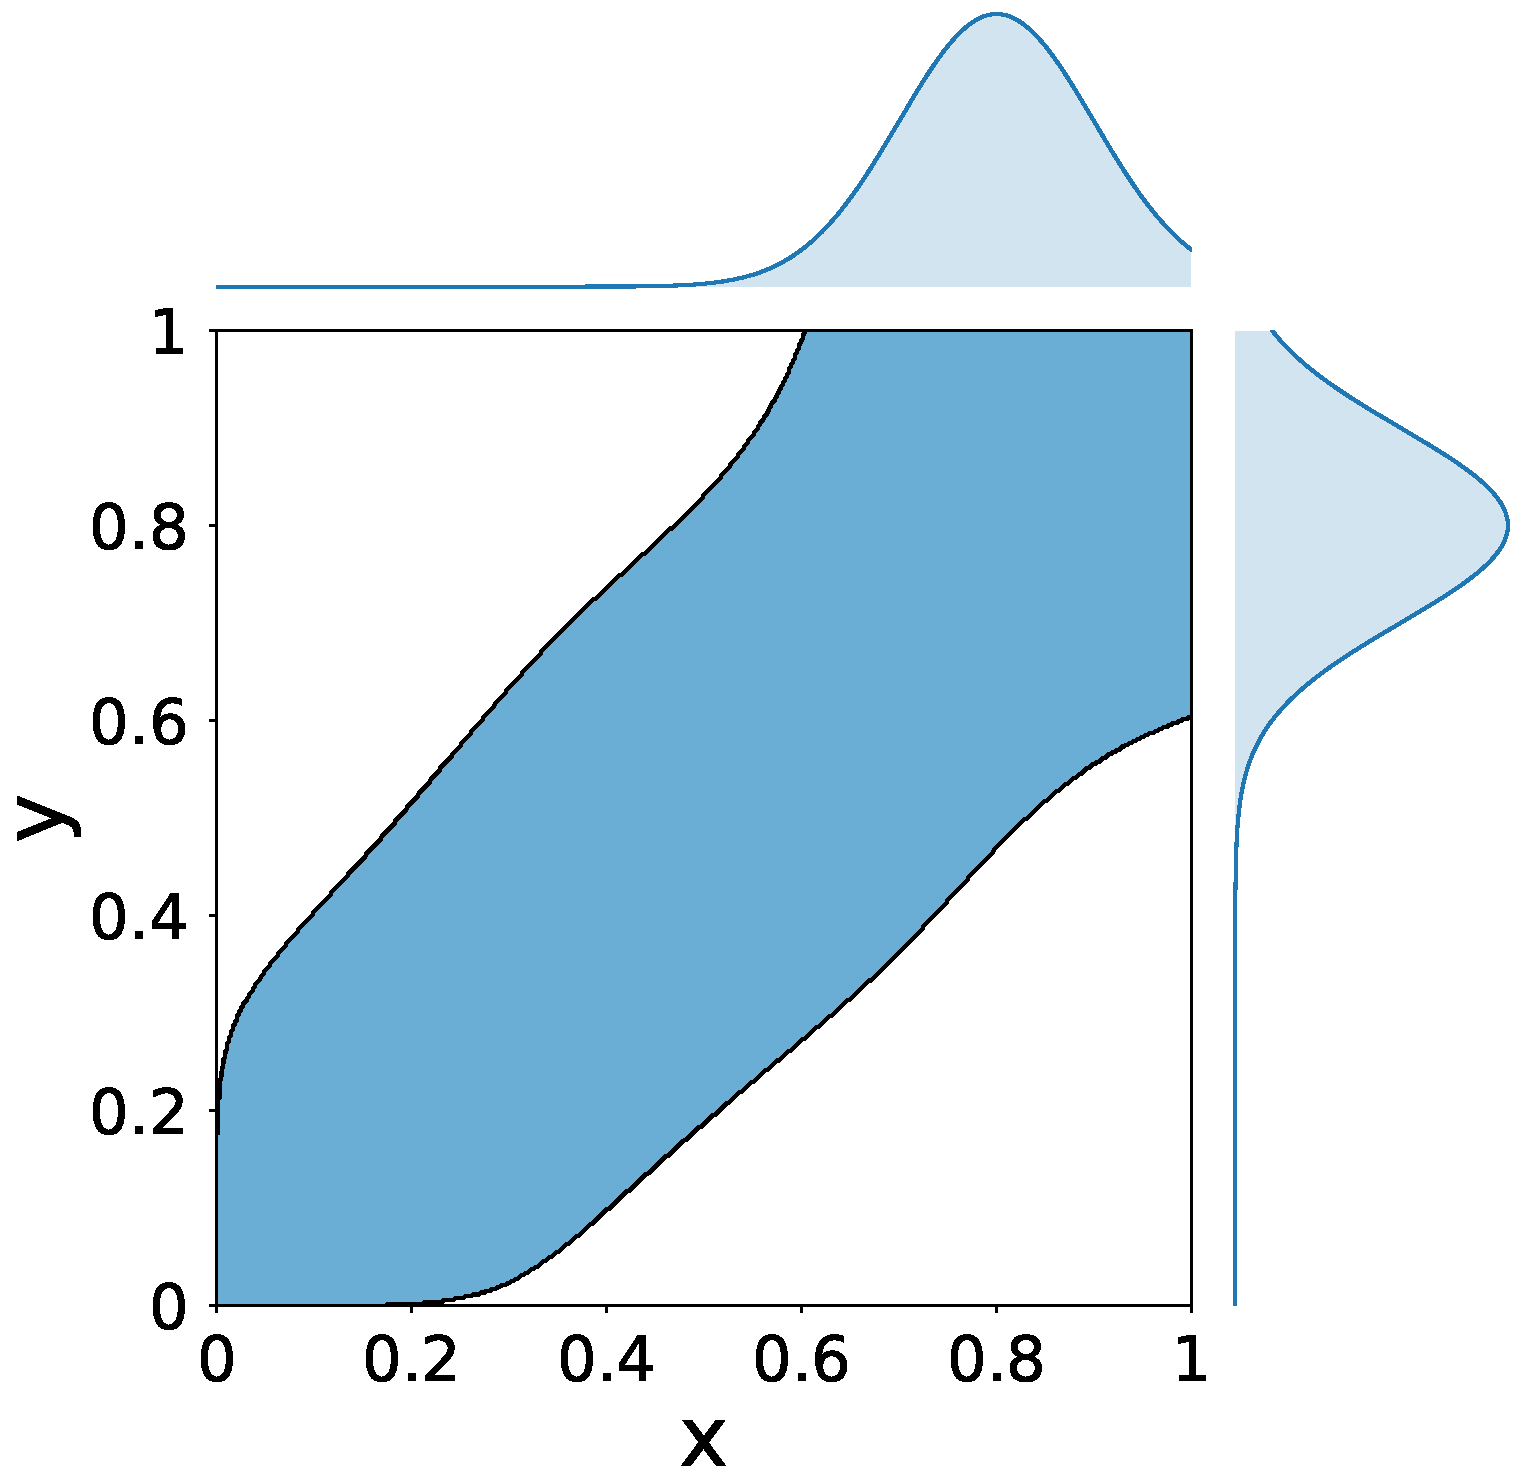
\includegraphics[scale=\smallScl]{fig4_6.pdf}}\\
	\raisebox{-2cm}{\rotatebox[origin=c]{90}{$\bm{\sigma=0.2}$}}\quad
	\subfloat{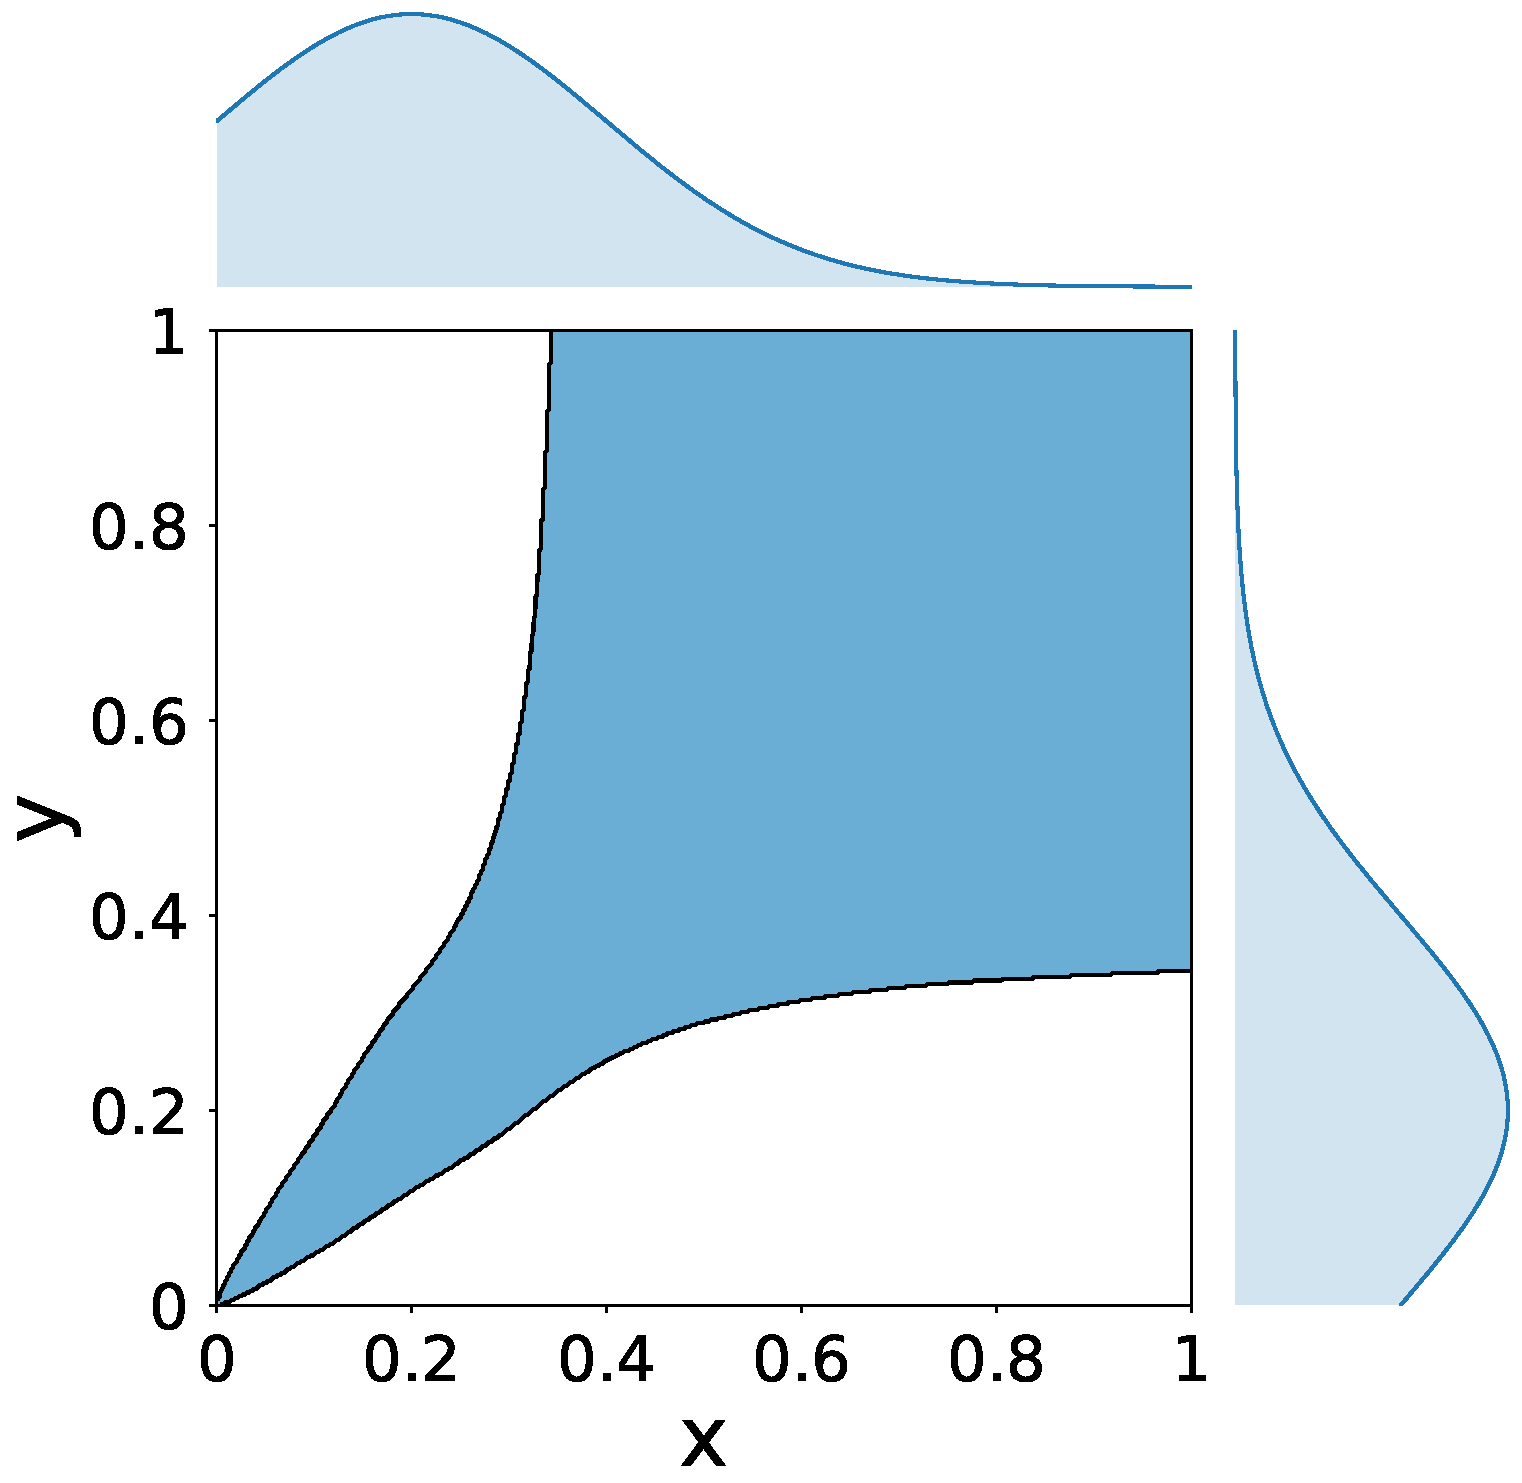
\includegraphics[scale=\smallScl]{fig4_7.pdf}}\quad
	\subfloat{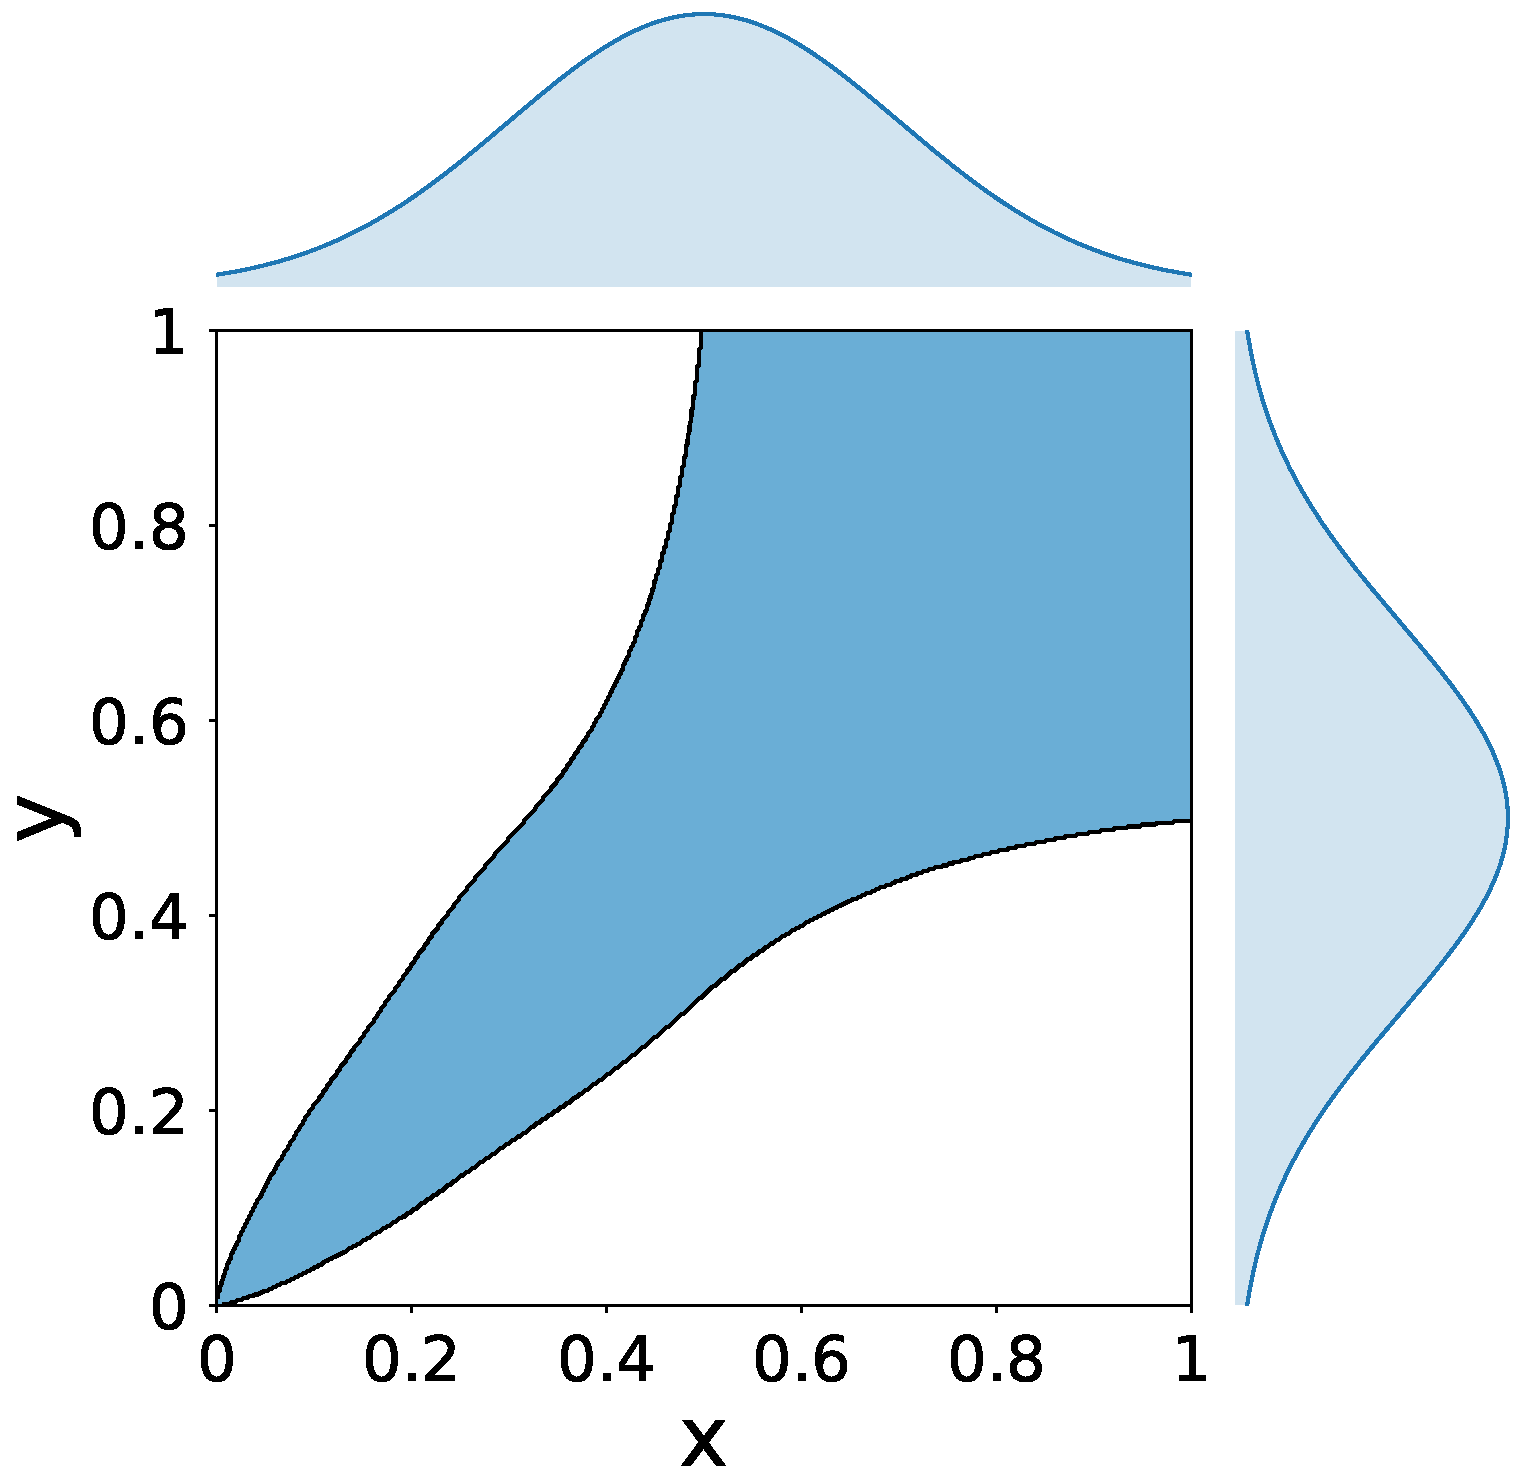
\includegraphics[scale=\smallScl]{fig4_8.pdf}}\quad
	\subfloat{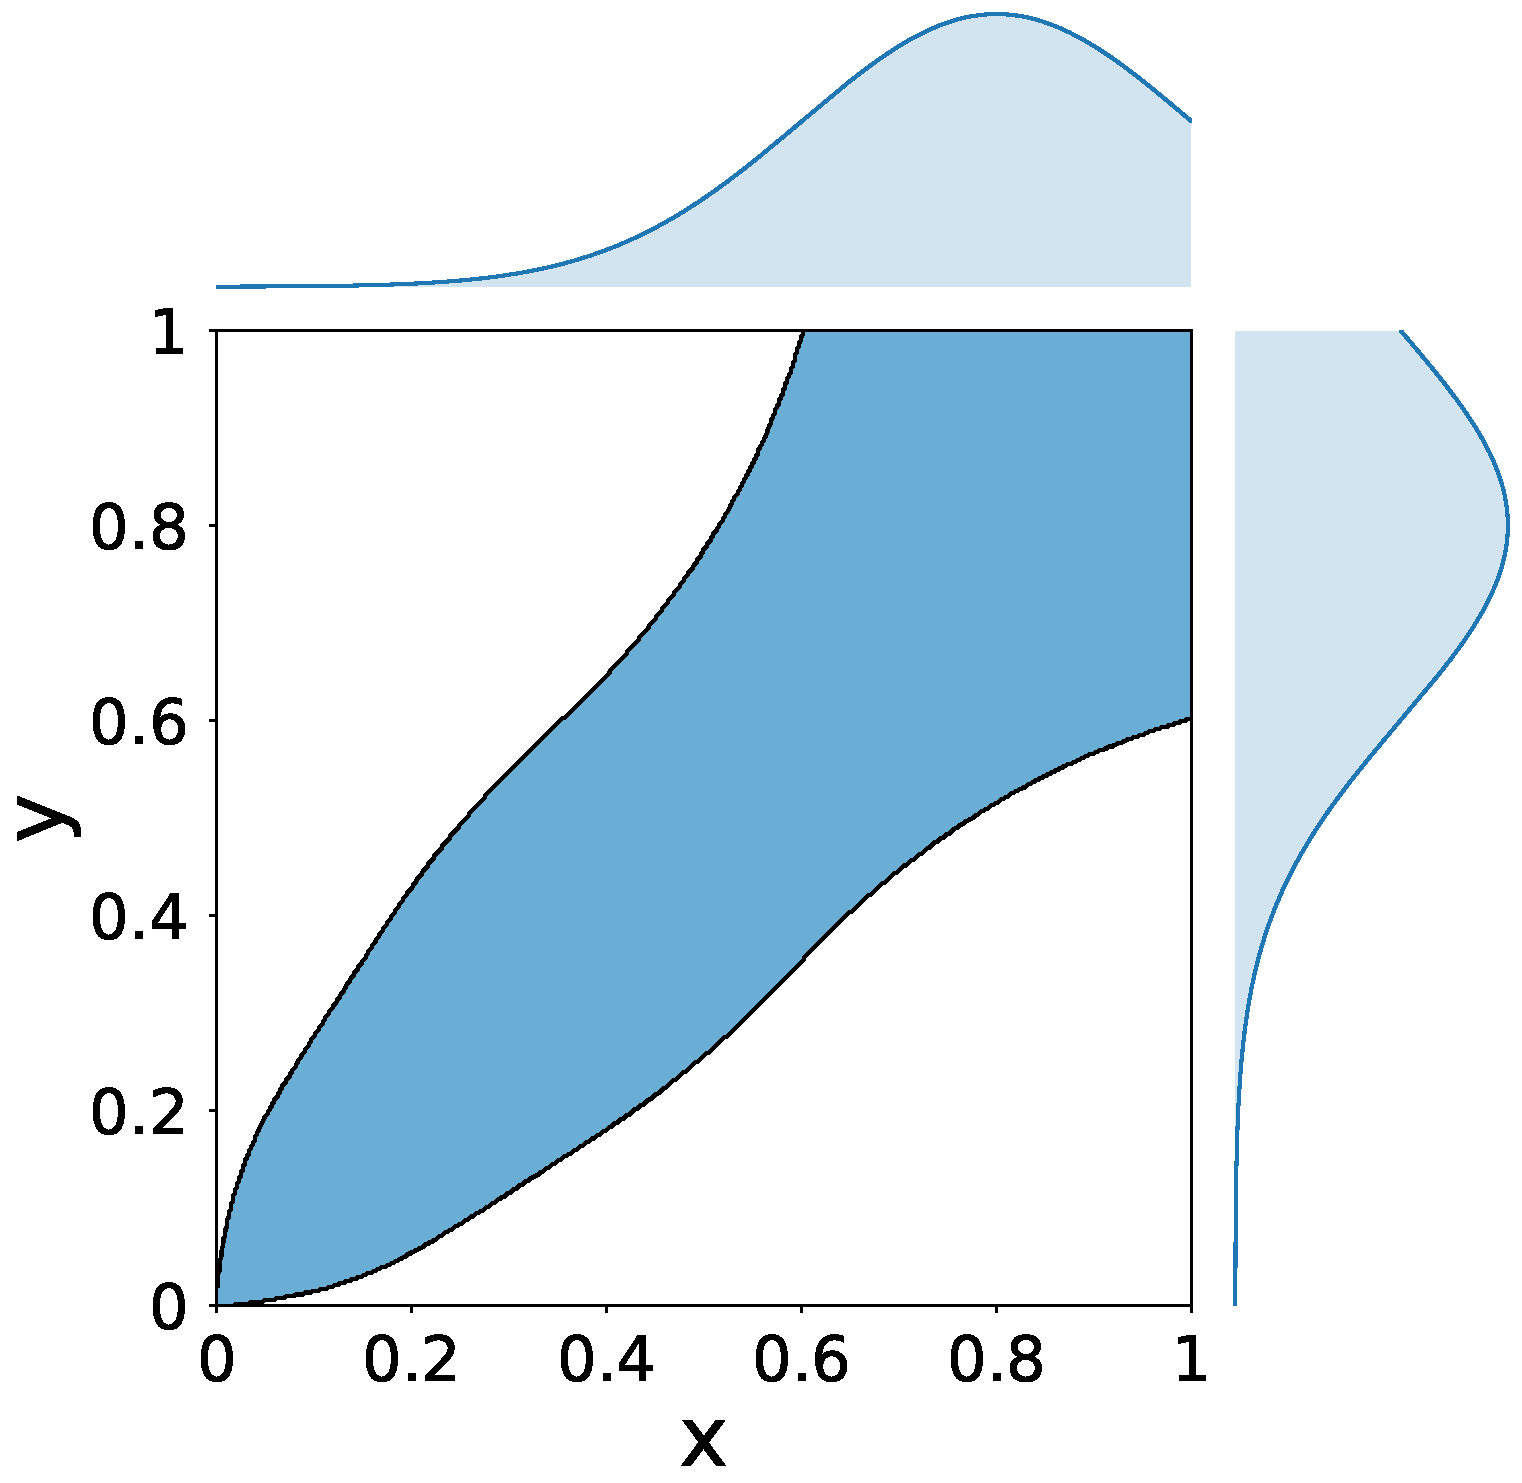
\includegraphics[scale=\smallScl]{fig4_9.pdf}}
	\caption{Matching set at the equilibrium for a Gaussian distribution of types. Results are shown for three values of the mean of the distribution $\mu \in \{0.2,0.5,0.8\}$ and for three values of the standard deviation $\sigma \in \{0.01,0.1,0.2\}$. The Gaussian distribution is truncated between 0 and 1. Parameters are $\delta=1 \ ; \ \rho=1000 \ ; \ r=1 \ ; \ f(x,y)=xy$.}
	\label{fig:fig4}
\end{figure}




\section*{Conclusion}
All the figures in the first reference article \citep{shimer_assortative_2000} have been successfully replicated (Fig.~\ref{fig:fig1} and \ref{fig:fig2}). Only one of the two figures in the second article \citep{smith_marriage_2006} has been replicated (Fig.~\ref{fig:fig3}A and \ref{fig:fig3}B). We have explored the possibility that our replication failure comes from an error in a parameter value given in a figure caption, yet, this is really uncertain, given that the same parameter value leads to a replication success for the second figure (Fig.~\ref{fig:fig3}C). We are unable to provide a clear explanation for this, since the code has been lost. This shows how important the archiving and replicating processes are, even for computational works. Finally, we have extended the algorithm to include additional assumptions about the distribution of types (Fig.~\ref{fig:fig4}) to match the current use of this algorithm in the search and matching literature. We hope this replication can help clarify the methods used in two papers of great importance, and that it can promote future research in the domain.


\section*{Acknowledgements}
We would like to thank Robert Shimer and Lones Smith for providing the code of one of the articles, and for useful information.
